\documentclass[11pt, a4paper]{article}
\usepackage[a4paper, margin=2.5cm]{geometry}
\usepackage[utf8]{inputenc}
\usepackage[T1]{fontenc}
\usepackage[spanish]{babel}
\usepackage{lmodern}
\usepackage{amsmath, amssymb, amsfonts, amsthm}
\usepackage{bm}
\usepackage{physics}
\usepackage{booktabs}
\usepackage{tabularx}
\usepackage{enumitem}
\usepackage{xcolor}
\usepackage{microtype}
\usepackage{float}
\usepackage{graphicx}
\usepackage{hyperref}

\hypersetup{
	colorlinks=true,
	linkcolor=blue!70!black,
	citecolor=blue!70!black,
	urlcolor=blue!70!black
}

\title{\textbf{Proyecto: Simulación del Problema Gravitacional de $N$ Cuerpos}\\
	\large Primer Proyecto para la Materia Astrofísica Computacional}
\author{\textbf{Zeuz Alejandro Espinosa Tobar}}
\date{9 de octubre de 2026}

\begin{document}

\maketitle

\hrule
\vspace{0.4cm}

\begin{abstract}
\noindent
Se desarrolla un motor de simulación gravitacional de $N$ cuerpos, construido desde cero
(sin bibliotecas de resolución de EDOs), que abarca las cuatro fases del proyecto:
formalismo de diferenciación numérica, integradores RK4 y simpléctico con detección de
eventos, simulación multi-etapa (benchmark Tierra-ISS con TLE real, sistema restringido
Tierra-Luna con puntos de Lagrange, y sistema solar interior 3D con Mercurio inclinado
$7^\circ$) y validación física mediante leyes de conservación y análisis formal del error
de truncamiento. El benchmark analítico mide una deriva de 84.9 m en 100 períodos
orbitales ($h = 15$ s) con escalado $h^{4.9}$, consistente con el orden global de RK4; el
integrador simpléctico conserva la energía por debajo de $4\times10^{-9}$ en 105\,000
pasos; y el análisis de precesión de Mercurio arroja $148.7''$/siglo en el modelo 3D
frente a $976.4''$/siglo en el planar, cuantificando la incidencia de los grados de
libertad fuera del plano.
\end{abstract}

\hrule

% ==============================================================================
\section{Fase I: Formalismo Matemático y Diferenciación Numérica}
% ==============================================================================

\subsection{Base Polinomial de Interpolación de Lagrange}

Consideremos una función $f(x)$ muestreada sobre una malla discreta compuesta por $n+1$ nodos equiespaciados $\{x_0, x_1, \dots, x_n\}$. La distancia constante entre nodos consecutivos se define como el paso de malla $h = x_{j+1} - x_j$.

Para expresar la posición de un punto continuo $x$ de forma adimensional, se introduce la transformación de variable $s$:
\begin{equation}
	x(s) = x_0 + s h \implies x - x_j = (s - j) h
	\label{eq:notacion}
\end{equation}

Sea el polinomio de interpolación de Lagrange de grado $n$, denotado como $P_n(x)$, definido como la combinación lineal de los valores de la función en los nodos $f_j = f(x_j)$:
\begin{equation}
	f(x) \approx P_n(x) = \sum_{j=0}^{n} l_j(x) f_j
	\label{eq:lagrange_poly}
\end{equation}
Donde la expresión explícita de la base es:
\begin{equation}
	l_j(x) = \frac{\pi(x)}{(x - x_j)\, \pi'(x_j)}
	\label{eq:base_lagrange_def}
\end{equation}
Aquí, $\pi(x)$ representa el \textit{Polinomio Productorio Nodal}, definido como:
\begin{equation}
	\pi(x) = \prod_{k=0}^{n} (x - x_k)
\end{equation}

Sustituyendo el cambio de variable $x - x_k = (s - k)h$, se reescribe el productorio en términos del parámetro adimensional $s$:
\begin{equation}
	\pi(s) = \prod_{k=0}^{n} (s - k)h = h^{n+1} \prod_{k=0}^{n} (s - k)
	\label{eq:productorio_s}
\end{equation}

Para evaluar el denominador de la Ec.~(\ref{eq:base_lagrange_def}), se halla la derivada de $\pi(x)$ respecto a $x$ evaluada explícitamente en el nodo $x_j$:
\begin{equation}
	\pi'(x_j) = \left. \frac{d\pi(x)}{dx} \right|_{x=x_j} = \left. \frac{ d \left( \prod_{k=0}^{n} (x - x_k) \right) }{dx} \right|_{x=x_j} = \prod_{\substack{k=0 \\ k \neq j}}^{n} (x_j - x_k)
\end{equation}

Sustituyendo $x_j - x_k = (j - k)h$:
\begin{align}
	\pi'(x_j) &= \prod_{\substack{k=0 \\ k \neq j}}^{n} (j - k)h \nonumber \\
	&= h^n \left[ \prod_{k=0}^{j-1} (j - k) \right] \cdot \left[ \prod_{k=j+1}^{n} (j - k) \right]
\end{align}
donde se separó el productorio en la parte anterior y posterior al término excluido $k=j$. Evaluando cada factor:
\begin{enumerate}
	\item El primer productorio es simplemente $j!$ (con el cambio de índice $i = j - k \implies i \in [1, j]$).
	\item El segundo productorio contiene $n-j$ términos negativos:
	      \begin{equation}
		      \prod_{k=j+1}^{n} (j - k) = (-1) \cdot (-2) \cdots (-(n-j)) = (-1)^{n-j} (n-j)!
	      \end{equation}
\end{enumerate}

Multiplicando ambas contribuciones se obtiene la forma cerrada:
\begin{equation}
	\pi'(x_j) = h^n (-1)^{n-j} j! (n-j)!
	\label{eq:pi_prime_node}
\end{equation}

\subsection{Deducción de la Fórmula General de Diferenciación Numérica de $n$ Puntos}

Para calcular la primera derivada $f'(x) \approx P_n'(x)$, se usa la regla de la cadena respecto a la variable adimensional $s$ (con $ds/dx = 1/h$):
\begin{equation}
	f'(x) = \frac{d P_n(x)}{dx} = \frac{1}{h} \frac{d}{ds} \left[ \sum_{j=0}^{n} l_j(s) f_j \right] = \frac{1}{h} \sum_{j=0}^{n} l_j'(s) f_j
	\label{eq:chain_rule_diff}
\end{equation}

Sustituyendo la Ec.~(\ref{eq:productorio_s}) y la Ec.~(\ref{eq:pi_prime_node}) en la definición de la base de Lagrange $l_j(s)$:
\begin{align}
	l_j(s) &= \frac{h^{n+1} \prod_{k=0}^{n} (s - k)}{(s - j)h \cdot h^n (-1)^{n-j} j! (n-j)!} \nonumber \\
	&= \frac{(-1)^{n-j}}{j! (n-j)!} \frac{\prod_{k=0}^{n} (s - k)}{s - j}
\end{align}

Definiendo el polinomio reducido $Q_j(s) = \dfrac{\prod_{k=0}^{n} (s-k)}{s-j}$ (polinomio de grado $n$ en $s$, pues el factor $(s-j)$ cancela el término correspondiente del productorio) y su expansión en potencias de $s$ mediante coeficientes algebraicos $a_{jk}$:
\begin{equation}
	Q_j(s) = \frac{1}{a_{jn}} \sum_{k=0}^{n} a_{jk} s^k
	\qquad \implies \qquad
	\frac{d Q_j(s)}{ds} = \frac{1}{a_{jn}} \sum_{k=1}^{n} k\, a_{jk} s^{k-1}
\end{equation}

Sustituyendo esta derivada dentro de la suma general de la Ec.~(\ref{eq:chain_rule_diff}) y aislando el término inicial $j=0$ de la sumatoria principal, se obtiene la \textbf{\textit{Fórmula General de Diferenciación Numérica de $n$ Puntos}}:
\begin{equation}
	f'(x) = \frac{1}{h} \left[ \frac{(-1)^{n}}{n! a_{0n}} \left( \sum_{k=1}^{n} k a_{0k} s^{k-1} \right) f_0 + \sum_{j=1}^{n} \left\{ \frac{(-1)^{n-j}}{j!(n-j)! a_{jn}} \left( \sum_{k=1}^{n} k a_{jk} s^{k-1} \right) \right\} f_j \right]
	\label{eq:general_num_diff}
\end{equation}

\subsection{Deducción de la Fórmula de 3 Puntos para la Primera Derivada ($n=2$)}

Considerando una plantilla (\textit{stencil}) de 3 puntos ($n=2$) definida por los nodos $x_0$, $x_1 = x_0 + h$ y $x_2 = x_0 + 2h$, se construyen explícitamente los tres polinomios de la base:
\begin{align}
	l_0(s) &= \frac{(s - 1)(s - 2)}{2} = \frac{s^2 - 3s + 2}{2} \\
	l_1(s) &= \frac{s (s - 2)}{-1} = -s^2 + 2s \\
	l_2(s) &= \frac{s (s - 1)}{2} = \frac{s^2 - s}{2}
\end{align}

Derivando cada base respecto a $s$:
\begin{align}
	\frac{d l_0}{ds} &= \frac{2s - 3}{2} \label{eq:dl0_ds} \\
	\frac{d l_1}{ds} &= 2(1 - s) \label{eq:dl1_ds} \\
	\frac{d l_2}{ds} &= \frac{2s - 1}{2} \label{eq:dl2_ds}
\end{align}

Sustituyendo en la regla de la cadena $f'(x) = \frac{1}{h} [ l_0' f_0 + l_1' f_1 + l_2' f_2 ]$:
\begin{equation}
	f'(x) = \frac{(-3 + 2s) f_0 + 4(1 - s) f_1 + (-1 + 2s) f_2}{2h}
	\label{eq:three_point_first_deriv}
\end{equation}

\subsection{La Diferencia Central Estándar como Caso Especial ($s=1$)}

\begin{proof}
	Para evaluar la derivada exactamente en el nodo central $x = x_1$, de $x = x_0 + sh$ se tiene $x_1 = x_0 + sh \implies s = 1$. Sustituyendo $s=1$ en la Ec.~(\ref{eq:three_point_first_deriv}):
	\begin{align}
		f'(x_1) &= \frac{(-3 + 2) f_0 + 4(0) f_1 + (-1 + 2) f_2}{2h} \nonumber \\
		&= \frac{-f_0 + f_2}{2h} = \frac{f_2 - f_0}{2h}
	\end{align}
	que es exactamente la fórmula estándar de diferencia finita central. \emph{Verificación numérica en código}: para $f(x) = \sin x$ con $h = 10^{-3}$, la función \texttt{primera\_derivada\_3\_puntos} con $s=1$ y la diferencia central producen resultados idénticos a precisión de máquina (error $1.27\times10^{-7}$ frente a $\cos(0.7)$ en ambos casos).
\end{proof}

\subsection{Segunda Derivada Numérica de 3 Puntos ($n=2$)}

Derivando la primera derivada mediante la regla de la cadena:
\begin{equation}
	f''(x) = \frac{d}{ds} \left[ \frac{1}{h} \sum_{j=0}^{2} l_j'(s) f_j \right] \frac{ds}{dx} = \frac{1}{h^2} \sum_{j=0}^{2} l_j''(s) f_j
\end{equation}
Con $l_0'' = 1$, $l_1'' = -2$, $l_2'' = 1$ (segunda derivada de las Ecs.~(\ref{eq:dl0_ds})--(\ref{eq:dl2_ds})):
\begin{equation}
	f''(x) = \frac{f_0 - 2f_1 + f_2}{h^2}
	\label{eq:second_deriv_formula}
\end{equation}

Ambas fórmulas están implementadas en el código y se \textbf{usan en la fase de validación}: aplicando la Ec.~(\ref{eq:second_deriv_formula}) a las posiciones registradas de la ISS se reproducen las aceleraciones newtonianas $\mathbf{a} = -\mu \mathbf{r}/r^3$ con un error relativo medio de $2.4\times10^{-5}$ (consistente con el error de truncamiento esperado $\sim \tfrac{2}{3}(h\omega)^2$ para $h\omega \approx 0.017$).

\subsection{Formulación Newtoniana del Problema de $N$ Cuerpos en Cartesianas 3D}

Para un sistema de $N$ masas puntuales con posiciones $\mathbf{x}_i(t) \in \mathbb{R}^3$, la fuerza neta sobre el cuerpo $i$ obedece la Ley de Gravitación Universal:
\begin{equation}
	\ddot{\mathbf{x}}_i = -G \sum_{\substack{j=0 \\ j \neq i}}^{N-1} \frac{m_j}{r_{ij}^3} \mathbf{r}_{ij}, \qquad \mathbf{r}_{ij} = \mathbf{x}_i - \mathbf{x}_j
	\label{eq:n_body_vector}
\end{equation}
con componentes cartesianas análogas en $x, y, z$. Para la propagación numérica se convierte el sistema de $N$ EDOs de segundo orden en $6N$ EDOs de primer orden con el vector de estado global $\mathbf{Y}_i = (\mathbf{x}_i, \mathbf{v}_i)^T \in \mathbb{R}^6$:
\begin{equation}
	\frac{d\mathbf{Y}_i}{dt} = \begin{pmatrix} \mathbf{v}_i \\ \mathbf{a}_i(\mathbf{x}_0, \dots, \mathbf{x}_{N-1}) \end{pmatrix}
	\label{eq:state_space_system}
\end{equation}

\subsection{Demostración de las Leyes de Conservación}

\subsubsection{Momento Lineal Total}
Con la segunda ley $m_i \ddot{\mathbf{q}}_i = \sum_{j\neq i}\mathbf{F}_{ij}$ y la tercera ley (fuerzas centrales por pares, $\mathbf{F}_{ji} = -\mathbf{F}_{ij}$):
\begin{equation}
	\frac{d\mathbf{P}}{dt} = \sum_{i=1}^n \sum_{j \neq i} \mathbf{F}_{ij} = \sum_{1 \le i < j \le n} (\mathbf{F}_{ij} + \mathbf{F}_{ji}) = \mathbf{0}
	\implies \mathbf{P}(t) = \text{cte.}
\end{equation}

\subsubsection{Energía Mecánica Total}
Con $T = \tfrac{1}{2}\sum_i m_i |\dot{\mathbf{q}}_i|^2$ y $V = \sum_{i<j} V_{ij}$, $-\dfrac{dV_{ij}}{dr} = f_{ij}(r)$:
\begin{equation}
	\frac{dT}{dt} = \sum_{1 \le i < j \le n} \mathbf{F}_{ij} \cdot (\dot{\mathbf{q}}_i - \dot{\mathbf{q}}_j), \qquad
	\frac{dV}{dt} = -\sum_{1 \le i < j \le n} \mathbf{F}_{ij} \cdot (\dot{\mathbf{q}}_i - \dot{\mathbf{q}}_j)
\end{equation}
Sumando ambas expresiones, $\dfrac{dE}{dt} = 0 \implies E(t) = \text{cte.}$

\subsubsection{Momento Angular Total}
Con $\mathbf{J} = \sum_i m_i (\mathbf{q}_i \times \dot{\mathbf{q}}_i)$ y agrupando por pares:
\begin{equation}
	\frac{d\mathbf{J}}{dt} = \sum_{1 \le i < j \le n} (\mathbf{q}_i - \mathbf{q}_j) \times \mathbf{F}_{ij} = \sum_{1 \le i < j \le n} \frac{f_{ij}}{|\mathbf{q}_i - \mathbf{q}_j|} \underbrace{\left[ (\mathbf{q}_i - \mathbf{q}_j) \times (\mathbf{q}_i - \mathbf{q}_j) \right]}_{= \, \mathbf{0}} = \mathbf{0}
\end{equation}
pues las fuerzas son centrales. Por tanto $\mathbf{J}(t) = \text{cte.}$

\subsection{Aproximación de Masa Puntual, Mareas y Clasificación de Sistemas}

La aproximación de masa puntual recupera las órbitas keplerianas analíticas pero desprecia efectos de tamaño finito (fuerzas de marea), responsables de fenómenos como la resonancia espín-órbita 3:2 de Mercurio, el incremento secular del semieje mayor lunar ($\sim 3.8$ cm/año) y las mareas oceánicas terrestres. En este proyecto todas las interacciones se modelan como masas puntuales, de modo que la comparación numérico-vs-analítica de la Tarea 1 mide \emph{exclusivamente} el error del integrador.

Siguiendo a Binney y Tremaine (2008), el tiempo de relajación de dos cuerpos
\begin{equation}
	t_{\text{relax}} \approx \frac{0.1\, N R}{\ln(N)\, v}
	\label{eq:t_relax}
\end{equation}
clasifica los sistemas en colisionales (cúmulos globulares, $t_{\text{relax}} \approx 400$ Ma) y no colisionales (halos de materia oscura, $t_{\text{relax}} \gg t_{\text{Hubble}}$). En los sistemas no colisionales se introduce una longitud de suavizado $\epsilon$ (potencial de Plummer) que mantiene la fuerza finita cuando $r_{ij} \to 0$:
\begin{equation}
	\mathbf{a}_i = -G \sum_{\substack{j=0 \\ j \neq i}}^{N-1} \frac{m_j \mathbf{r}_{ij}}{\left(r_{ij}^2 + \epsilon^2\right)^{3/2}}
	\label{eq:softened_acc}
\end{equation}
El módulo de fuerzas del código implementa la Ec.~(\ref{eq:softened_acc}) con parámetro $\epsilon$ configurable. En este proyecto se usa $\epsilon = 0$ (ley newtoniana exacta) porque los sistemas simulados son jerárquicos y no colisionales en la práctica: no se producen encuentros cercanos entre pares, y el suavizado degradaría precisamente el benchmark analítico de la Tarea 1, que exige el potencial kepleriano exacto.

% ==============================================================================
\section{Fase II: Arquitectura del Motor de Simulación y Solucionadores de EDO}
% ==============================================================================

El motor se desarrolla desde cero, sin bibliotecas externas de resolución de EDOs (únicamente \texttt{NumPy} para aritmética de arreglos y \texttt{Matplotlib} para visualización).

\subsection{Integradores Numéricos: RK4 y Método Simpléctico}

\subsubsection{Runge-Kutta de 4.º Orden (RK4)}
Error local $O(h^5)$ y global $O(h^4)$. Dado el estado $\mathbf{Y}(t)$:
\begin{equation}
	\mathbf{Y}_{n+1} = \mathbf{Y}_n + \frac{h}{6} \left(\mathbf{k}_1 + 2\mathbf{k}_2 + 2\mathbf{k}_3 + \mathbf{k}_4\right)
\end{equation}
con las pendientes intermedias estándar $\mathbf{k}_1 = \mathbf{f}(t_n, \mathbf{Y}_n)$, $\mathbf{k}_2 = \mathbf{f}(t_n + \tfrac{h}{2}, \mathbf{Y}_n + \tfrac{h}{2}\mathbf{k}_1)$, etc. Es el integrador de las Tareas 1 y 2.

\subsubsection{Integrador Simpléctico (Verlet velocidad, KDK)}
Esquema de segundo orden que conserva el volumen en el espacio de fases y acota la deriva del Hamiltoniano:
\begin{align}
	\mathbf{v}_i\left(t + \tfrac{h}{2}\right) &= \mathbf{v}_i(t) + \tfrac{h}{2}\,\mathbf{a}_i\bigl(\mathbf{x}(t)\bigr) \\
	\mathbf{x}_i(t+h) &= \mathbf{x}_i(t) + h\,\mathbf{v}_i\left(t+\tfrac{h}{2}\right) \\
	\mathbf{v}_i(t+h) &= \mathbf{v}_i\left(t+\tfrac{h}{2}\right) + \tfrac{h}{2}\,\mathbf{a}_i\bigl(\mathbf{x}(t+h)\bigr)
\end{align}
Es el integrador de la Tarea 3 (larga duración). La Fase IV muestra numéricamente el contraste de propiedades de conservación entre ambos esquemas.

\subsection{Ecuación de Kepler, Solver Iterativo y Elementos Orbitales}
\label{sec:kepler_solver}

La solución analítica del problema de dos cuerpos requiere resolver la ecuación trascendental de Kepler
\begin{equation}
	M = E - e\sin E, \qquad M(t) = M_0 + n\,t, \qquad n = \sqrt{\mu/a^3}
	\label{eq:kepler_eq}
\end{equation}
que se resuelve por iteración de Newton-Raphson,
\begin{equation}
	E_{k+1} = E_k - \frac{E_k - e\sin E_k - M}{1 - e\cos E_k}
\end{equation}
hasta converger (tolerancia $10^{-12}$). La posición y velocidad en el plano orbital se obtienen con la anomalía verdadera
\begin{equation}
	\nu = 2\arctan_2\!\left(\sqrt{1+e}\,\sin\tfrac{E}{2},\; \sqrt{1-e}\,\cos\tfrac{E}{2}\right), \qquad
	r = a(1 - e\cos E)
\end{equation}
\begin{equation}
	\mathbf{r}_{\text{orb}} = r(\cos\nu, \sin\nu, 0), \qquad
	\mathbf{v}_{\text{orb}} = \frac{\mu}{h}\left(-\sin\nu,\; e + \cos\nu,\; 0\right), \quad h = \sqrt{\mu a (1-e^2)}
\end{equation}
y se transforman al marco inercial mediante la rotación $\mathbf{Q} = R_3(\Omega)\,R_1(i)\,R_3(\omega)$.

El código incluye además un \textbf{parser de TLE} que extrae directamente los elementos $a$ (vía $a = (\mu/n^2)^{1/3}$ con el movimiento medio del TLE), $e$, $i$, $\Omega$, $\omega$ y $M_0$. Este módulo alimenta tanto las condiciones iniciales de la Tarea 1 como la \textbf{solución analítica de referencia} contra la cual se mide la deriva del solver. A la inversa, la función \texttt{elementos\_osculantes} recupera $(a, e, i, \Omega, \omega, \varpi)$ desde vectores de estado cartesianos (productos cruz $\mathbf{h} = \mathbf{r}\times\mathbf{v}$ y vector excentricidad), y es la herramienta del análisis de precesión de la Tarea 3.

\subsection{Detección de Eventos: Interpolación de Lagrange + Bisección}

Cuando el paso $h$ es demasiado grueso para capturar un evento (cruce de un plano orbital, $\mathbf{r}\cdot\mathbf{v} = 0$ en los ápsides), el estado se interpola entre pasos con la base de Lagrange sobre nodos vecinos:
\begin{equation}
	\mathbf{Y}(t) = \sum_{j=0}^{n} l_j(t)\, \mathbf{Y}_j, \qquad l_j(t) = \prod_{\substack{k=0 \\ k \neq j}}^{n} \frac{t - t_k}{t_j - t_k}
\end{equation}
y el instante exacto del evento se aísla con el método de bisección (teorema de Bolzano): se evalúa el punto medio $t_m$, se conserva el subintervalo con cambio de signo y se itera hasta $|t_b - t_a| < \text{tol}$.

\textbf{Verificación exigida por el enunciado}: para la función de prueba unit-normalizada $g(x) = x^3 - 2.667^3$ en $[0, 5]$, la rutina detecta la constante de cruce
\begin{center}
	\texttt{raíz = 2.667000000000} \quad (error $< 10^{-9}$, verificación \texttt{PASA})
\end{center}
Este verificador se ejecuta como \texttt{assert} al inicializar el notebook.

\subsection{Requisitos del Código}

\begin{itemize}
	\item \textbf{Modularidad}: el potencial/aceleración (Ec.~\ref{eq:softened_acc}) es un módulo independiente de los integradores; RK4 y Verlet son intercambiables por parámetro.
	\item \textbf{Vectorización 3D}: posiciones y velocidades como arreglos $(N, 3)$; las sumas sobre cuerpos se evalúan con operaciones vectoriales de \texttt{NumPy}.
	\item \textbf{Registro temporal (\textit{timestamped logging})}: en \emph{cada paso} se guardan $t$, la matriz de posiciones, la matriz de velocidades, la energía total $E(t)$ y los momentos $\mathbf{L}(t)$ y $\mathbf{P}(t)$. Este registro se activa en las tres tareas.
\end{itemize}

% ==============================================================================
\section{Fase III: Tareas de Simulación Multi-Etapa}
% ==============================================================================

\subsection{Tarea 1: Benchmark Analítico de 2 Cuerpos (Tierra + ISS)}

\subsubsection{Condiciones iniciales desde TLE}
El sistema se inicializa con los elementos de un \textbf{TLE real y reciente} de la ISS (ZARYA, NORAD 25544), obtenido de Celestrak con época del 9 de octubre de 2026 (19:42 UTC):

\begin{table}[H]
	\centering
	\begin{tabular}{lrlr}
		\toprule
		Elemento & Valor & Derivado & Valor \\
		\midrule
		Semieje mayor $a$ & $6\,798.393$ km & Período $T = 2\pi/n$ & $92.98$ min \\
		Excentricidad $e$ & $0.0006775$ & Perigeo $a(1-e)$ & $6\,793.787$ km \\
		Inclinación $i$ & $51.6314^\circ$ & Apogeo $a(1+e)$ & $6\,802.999$ km \\
		$\Omega, \omega, M_0$ & $92.7969^\circ, 242.6225^\circ, 117.4075^\circ$ & Movimiento medio $n$ & $15.48793$ rev/día \\
		\bottomrule
	\end{tabular}
	\caption{Elementos orbitales extraídos del TLE de la ISS (época 2026-10-09).}
	\label{tab:tle}
\end{table}

El estado inicial se genera con el módulo de la Sección~\ref{sec:kepler_solver} y se traslada al marco baricéntrico. Nota de consistencia numérica: la masa terrestre del código se define como $M_\oplus = \mu_\oplus/G$ con $\mu_\oplus = 3.986004418\times10^{14}\ \mathrm{m^3/s^2}$ (la constante con la que se reducen los TLE); usar en cambio $G \times 5.972\times10^{24}$ introduce una inconsistencia relativa $\Delta\mu/\mu \approx 2.8\times10^{-5}$ que produce un desfase sistemático de $\sim$240 km en 100 órbitas, ajeno por completo al error del integrador.

\subsubsection{Deriva del solver frente a la solución analítica}
Se propaga el sistema con RK4 ($h = 15$ s) durante \textbf{100 períodos orbitales} ($6.46$ días) y se compara contra la solución Kepleriana exacta propagada con el solver de la Sección~\ref{sec:kepler_solver}:
\begin{equation}
	\text{drift}(t) = \left\| \mathbf{r}_{\text{num}}(t) - \mathbf{r}_{\text{Kepler}}(t) \right\|
\end{equation}

\begin{figure}[H]
	\centering
	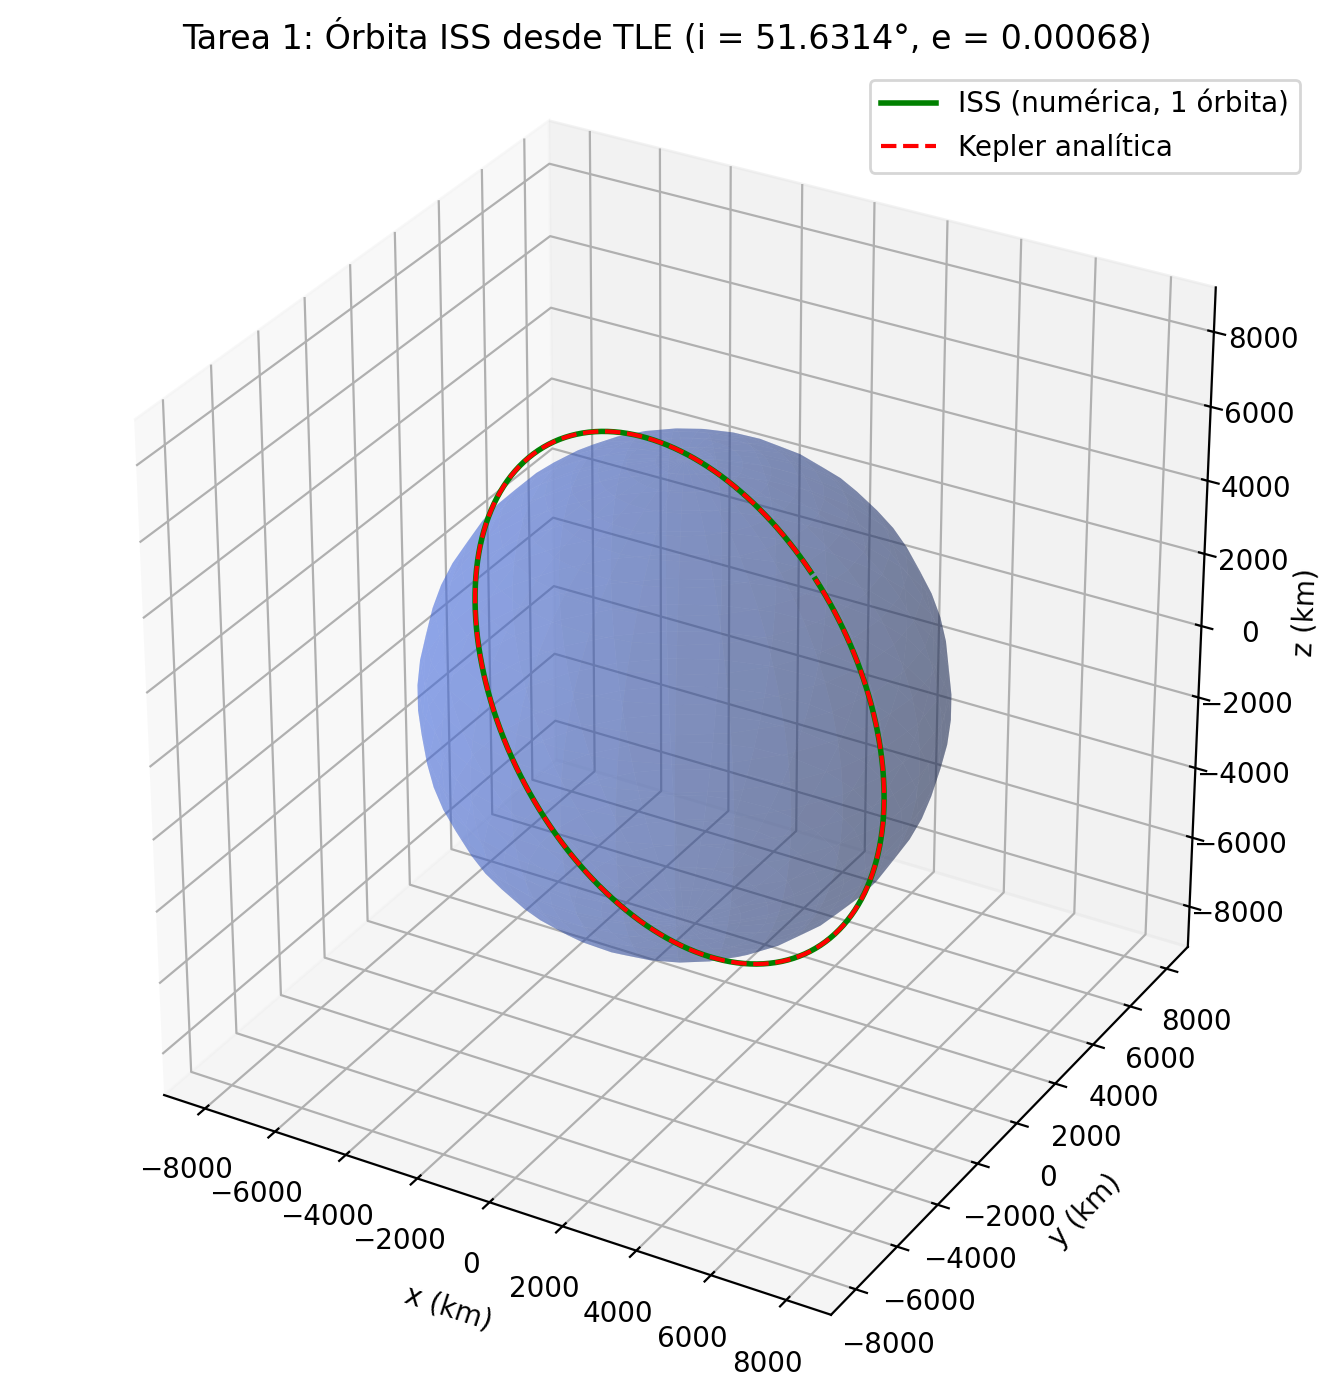
\includegraphics[width=0.62\textwidth]{T1v2_01_Orbita_3D.png}
	\caption{Tarea 1: órbita de la ISS durante un período desde el TLE real ($i = 51.63^\circ$). La trayectoria numérica (verde) y la analítica (roja, discontinua) son indistinguibles a esta escala.}
	\label{fig:t1_orbita}
\end{figure}

\begin{figure}[H]
	\centering
	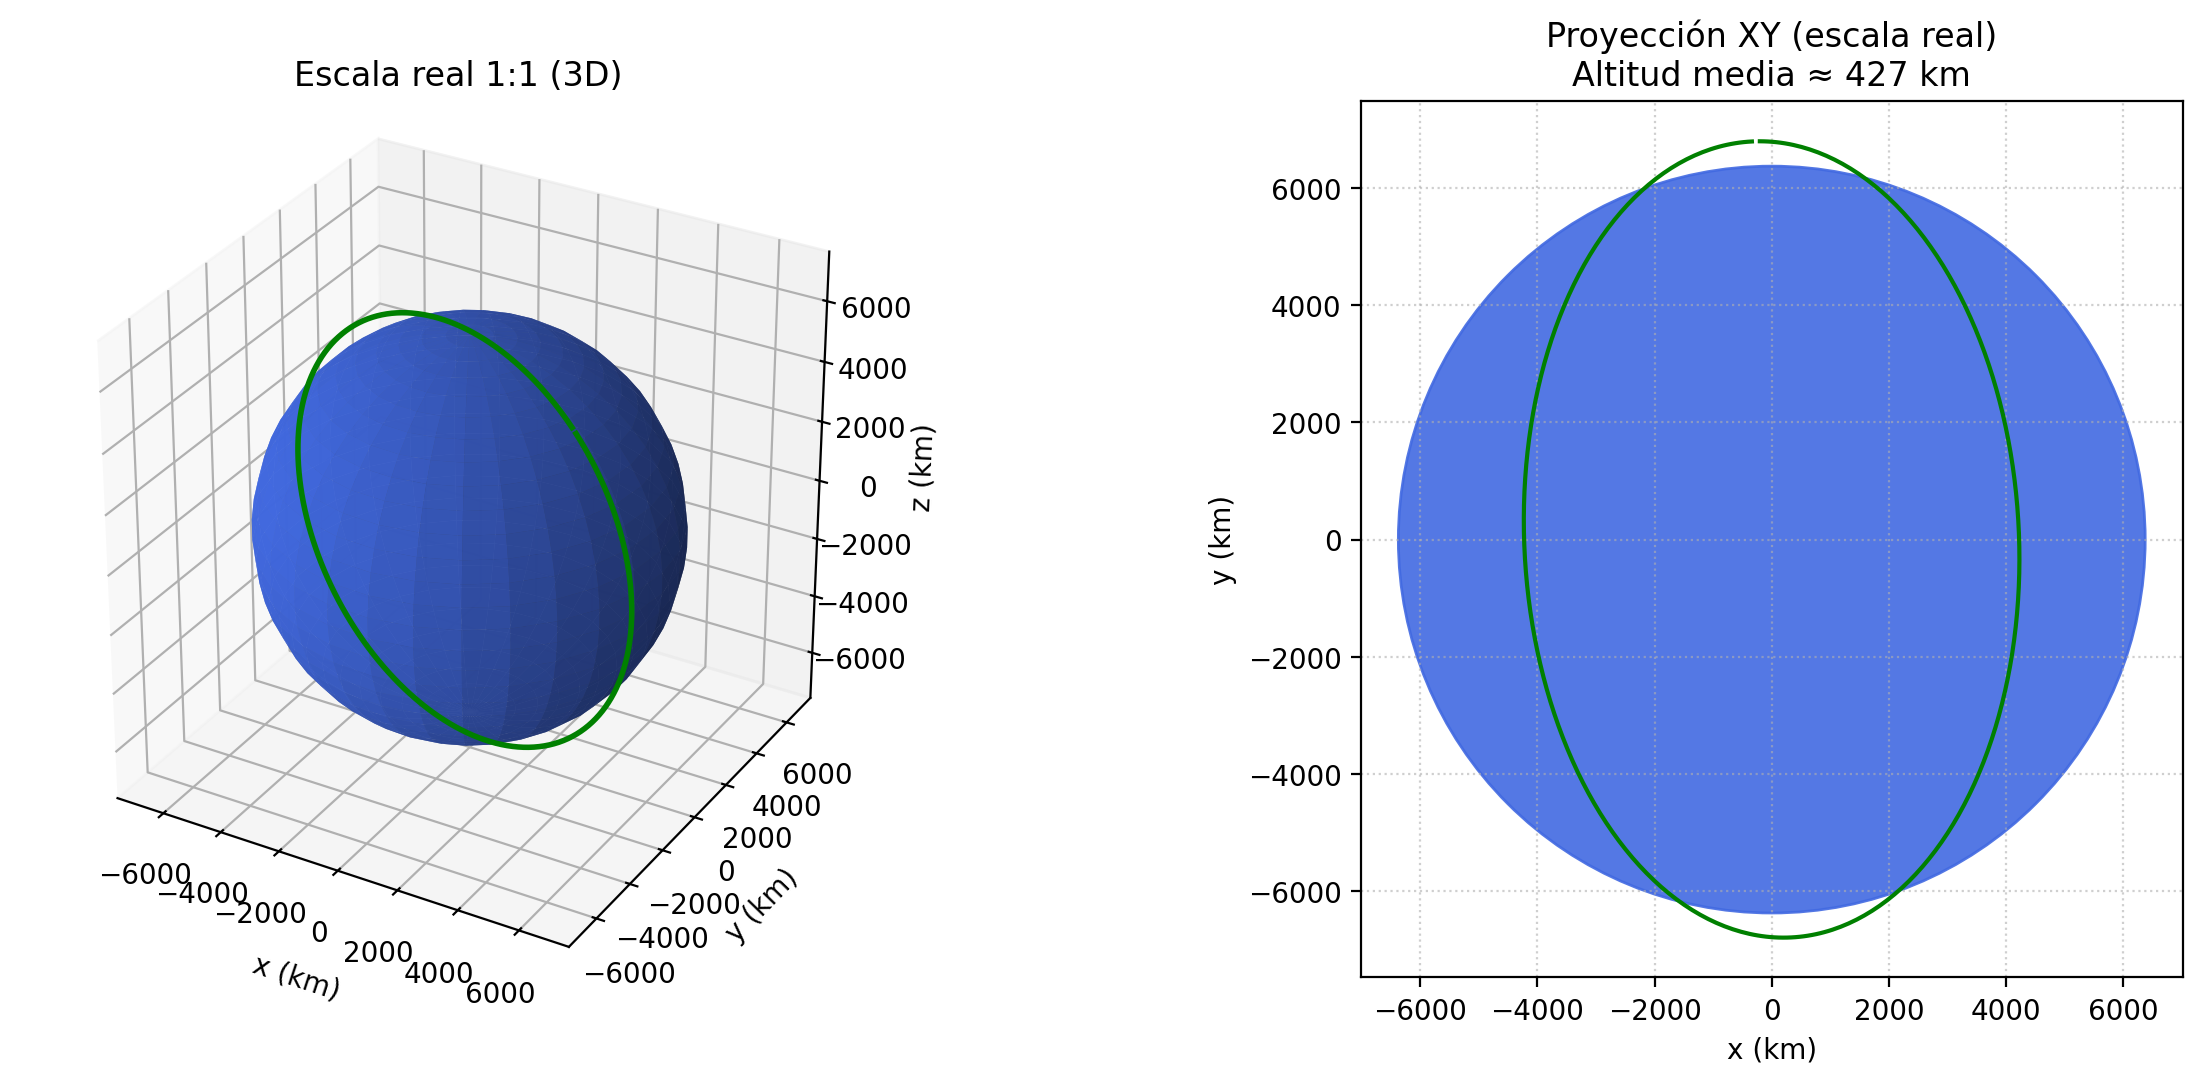
\includegraphics[width=0.95\textwidth]{T1v2_06_Escala_Real.png}
	\caption{Tarea 1: escala real $1{:}1$ (3D y proyección XY) con la Tierra a su tamaño verdadero. La órbita LEO ($a = 6\,798$ km) apenas roza la superficie ($R_\oplus = 6\,371$ km): la altitud de $\sim$430 km es apenas el $6.7\%$ del radio terrestre.}
	\label{fig:t1_escala}
\end{figure}

\begin{figure}[H]
	\centering
	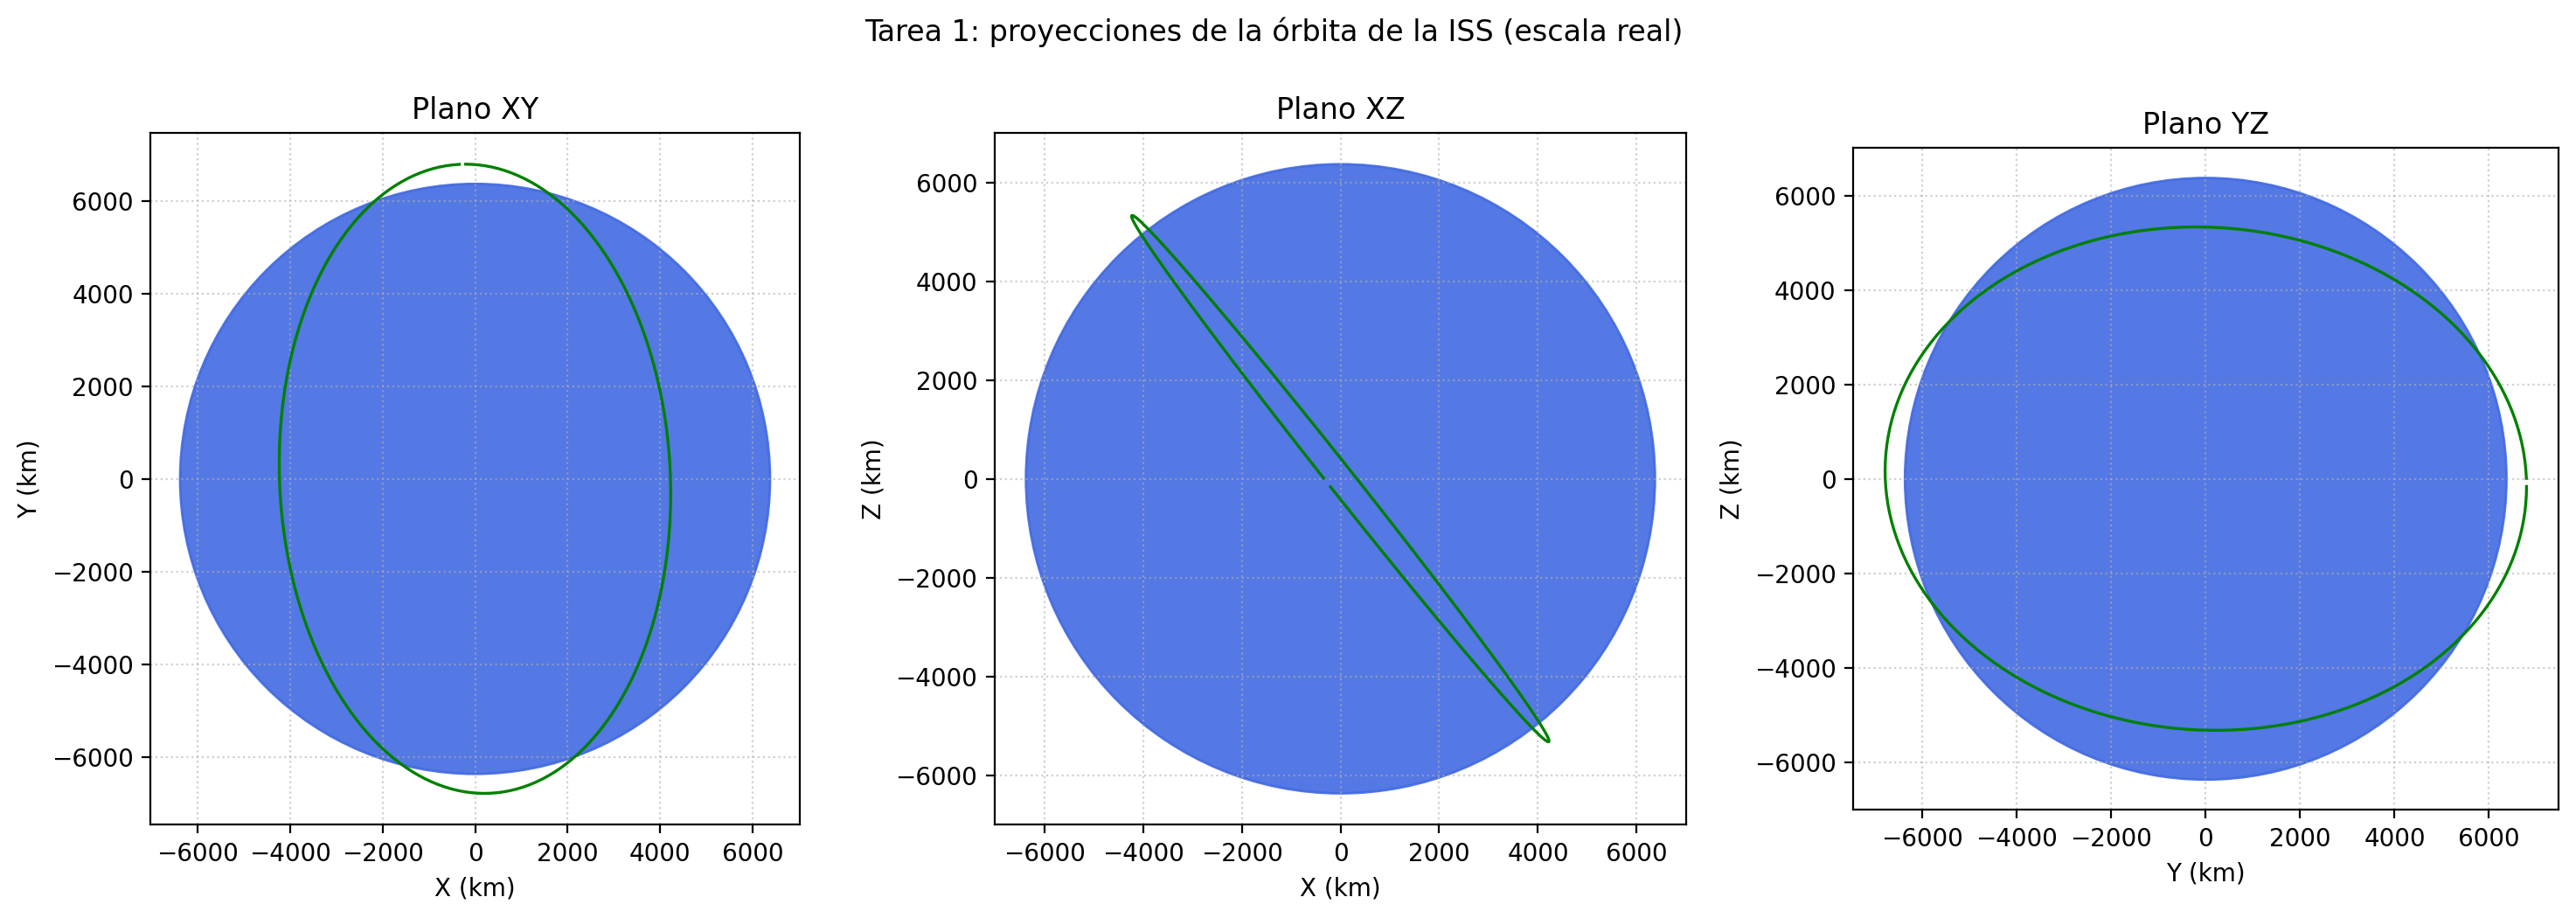
\includegraphics[width=0.98\textwidth]{T1v2_07_Planos.png}
	\caption{Tarea 1: proyecciones de la órbita de la ISS sobre los tres planos (escala real). La inclinación de $51.63^\circ$ del TLE se manifiesta como la amplitud de la oscilación en los planos XZ y YZ.}
	\label{fig:t1_planos}
\end{figure}

\begin{figure}[H]
	\centering
	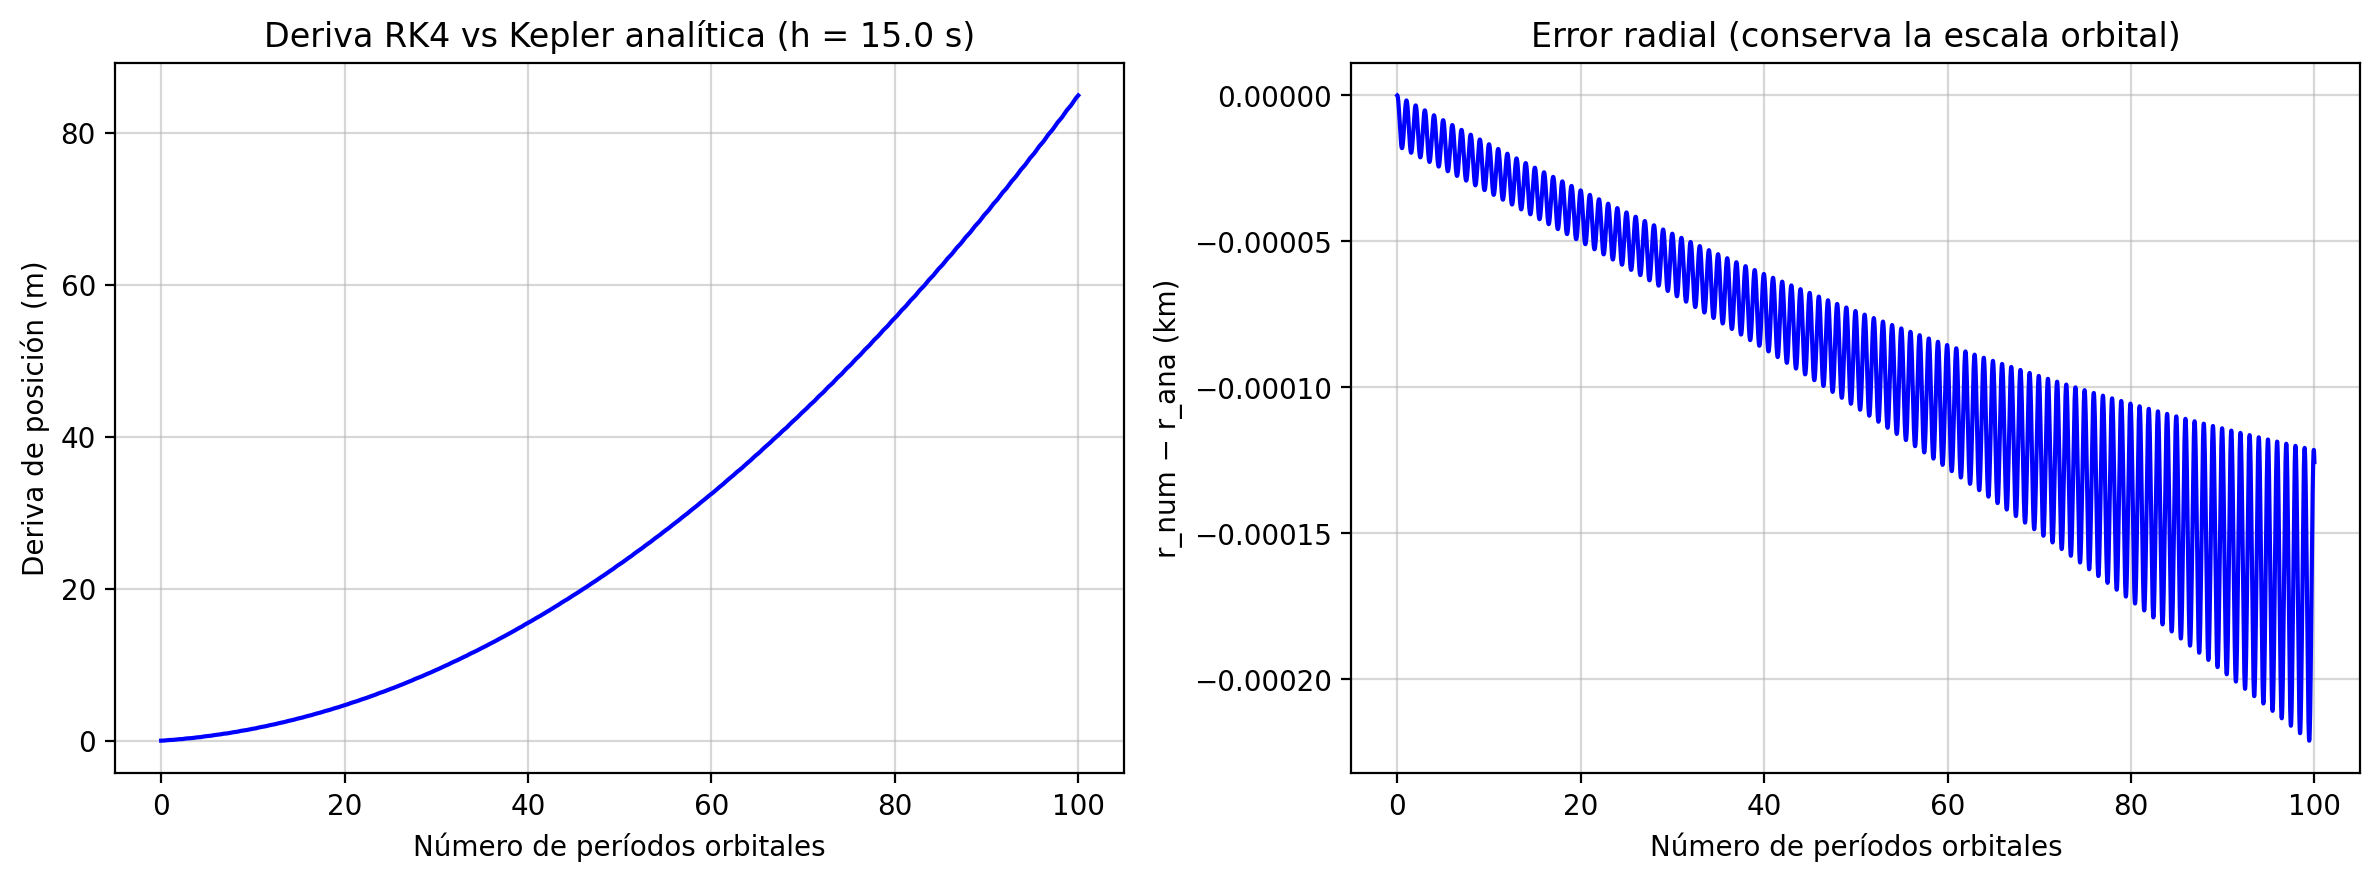
\includegraphics[width=0.95\textwidth]{T1v2_02_Deriva_100T.png}
	\caption{Tarea 1: deriva de posición RK4 vs.\ solución Kepleriana durante 100 períodos (izquierda) y error radial (derecha). La deriva crece secularmente hasta $84.9$ m con $h = 15$ s.}
	\label{fig:t1_deriva}
\end{figure}

La deriva final medida es de $\mathbf{84.9\ m}$ con $h = 15$ s, con crecimiento aproximadamente lineal en el tiempo, característico de un integrador no simpléctico de precisión alta: el error de fase local se acumula de forma secular a lo largo de las $\sim$37\,000 pasos. El error radial, en cambio, permanece acotado a escalas de centímetros: la órbita conserva su geometría y el error se manifiesta casi por completo como desfase along-track.

\subsubsection{Detección de eventos: ápsides con Lagrange + bisección}
Se detectaron los ápsides ($\mathbf{r}\cdot\mathbf{v} = 0$) interpolando el estado sub-paso con plantillas de Lagrange de 4 nodos y refinando con bisección. Resultados: \textbf{200 ápsides} (100 perigeos, 100 apogeos), espaciado medio $2\,789.27$ s frente al teórico $T/2 = 2\,789.27$ s (error medio $< 10^{-3}$ s), con radios medios de perigeo $6\,793.787$ km y apogeo $6\,802.999$ km, que reproducen \emph{exactamente} los valores $a(1\mp e)$ del TLE. Esta prueba valida conjuntamente la interpolación, el detector de eventos y la propia integración.

\begin{figure}[H]
	\centering
	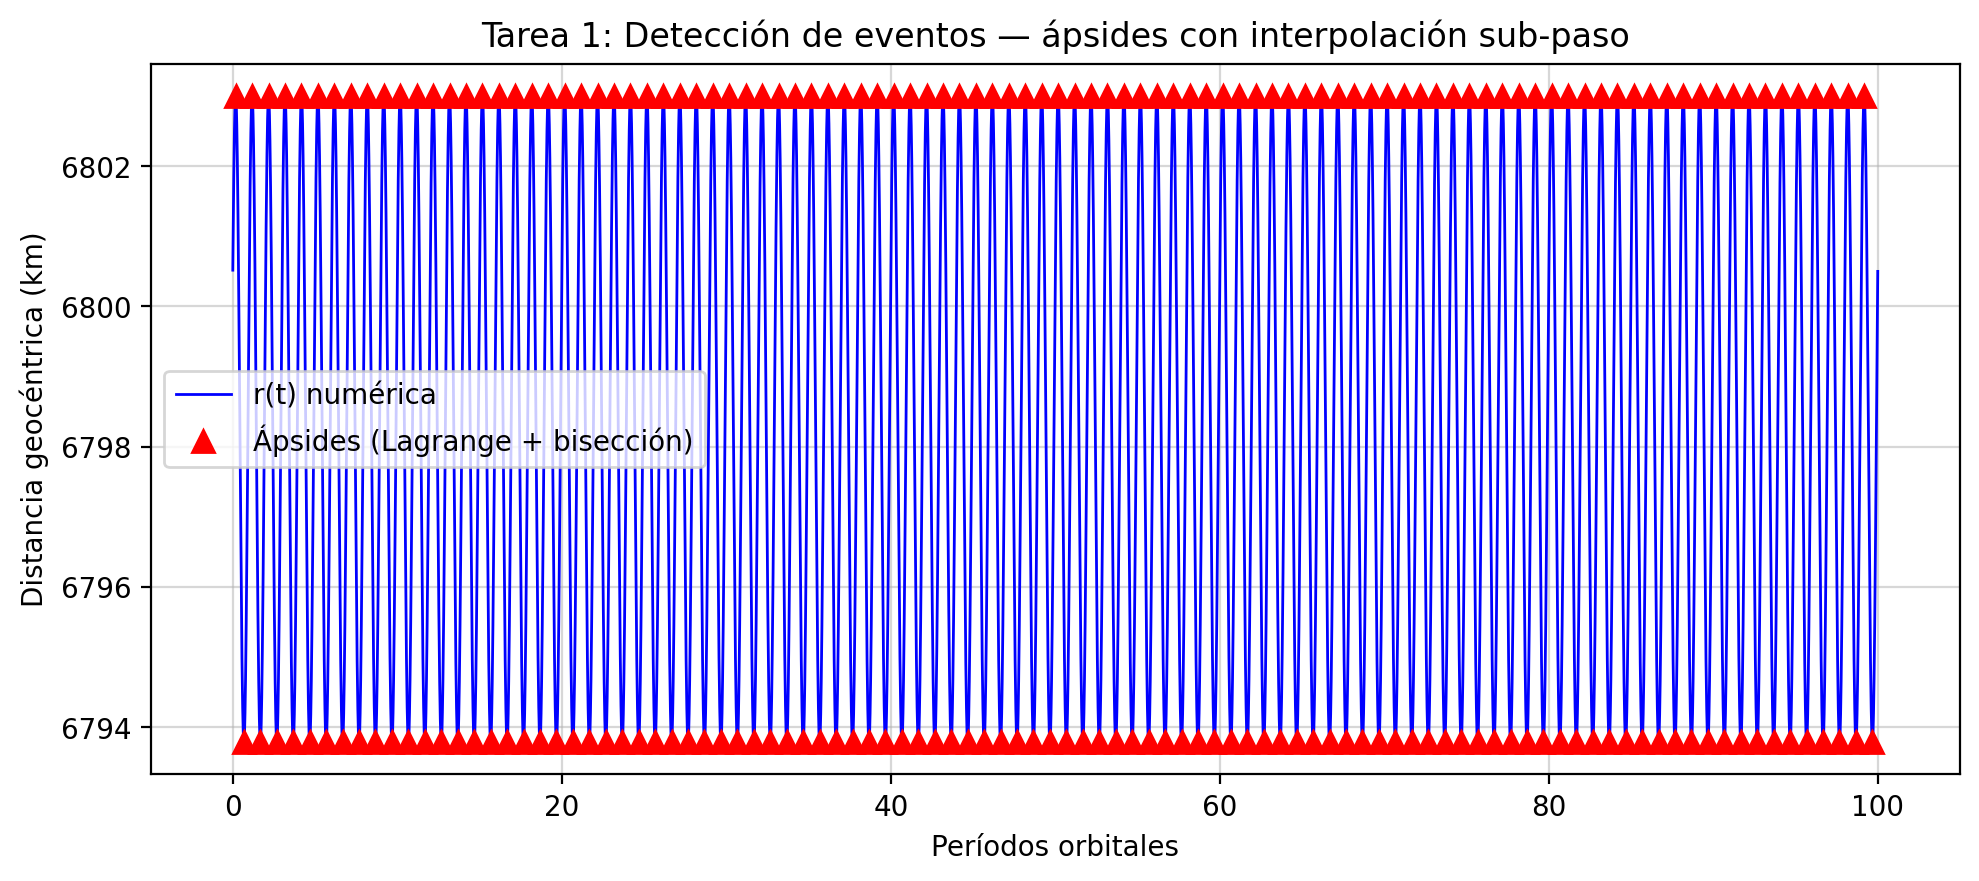
\includegraphics[width=0.85\textwidth]{T1v2_05_Apsides.png}
	\caption{Tarea 1: ápsides detectados (triángulos) sobre la curva $r(t)$ mediante interpolación de Lagrange + bisección.}
	\label{fig:t1_apsides}
\end{figure}

\subsection{Tarea 2: Sistema Restringido y Puntos de Lagrange}

Se modela un sistema de \textbf{5 cuerpos}: Tierra y Luna en órbita circular baricéntrica exacta, un satélite en LEO circular de 400 km (analógico a la ISS), un satélite tipo JWST en $L_2$ del sistema Tierra-Luna, y un \textbf{satélite de prueba en $L_4$}. La posición de $L_2$ se sitúa más allá de la Luna a
\begin{equation}
	\Delta r_{L_2} = D_{TL} \left[ \left(\tfrac{q}{3}\right)^{1/3} + 1 \right] \approx 68\,800\ \mathrm{km}, \qquad q = \frac{M_L}{M_T},
\end{equation}
 El satélite de $L_4$ se coloca por rotación de $60^\circ$ del vector Tierra$\to$Luna (posiciones y velocidades). Integración: RK4, $h = 15$ s, 28 días.

\begin{figure}[H]
	\centering
	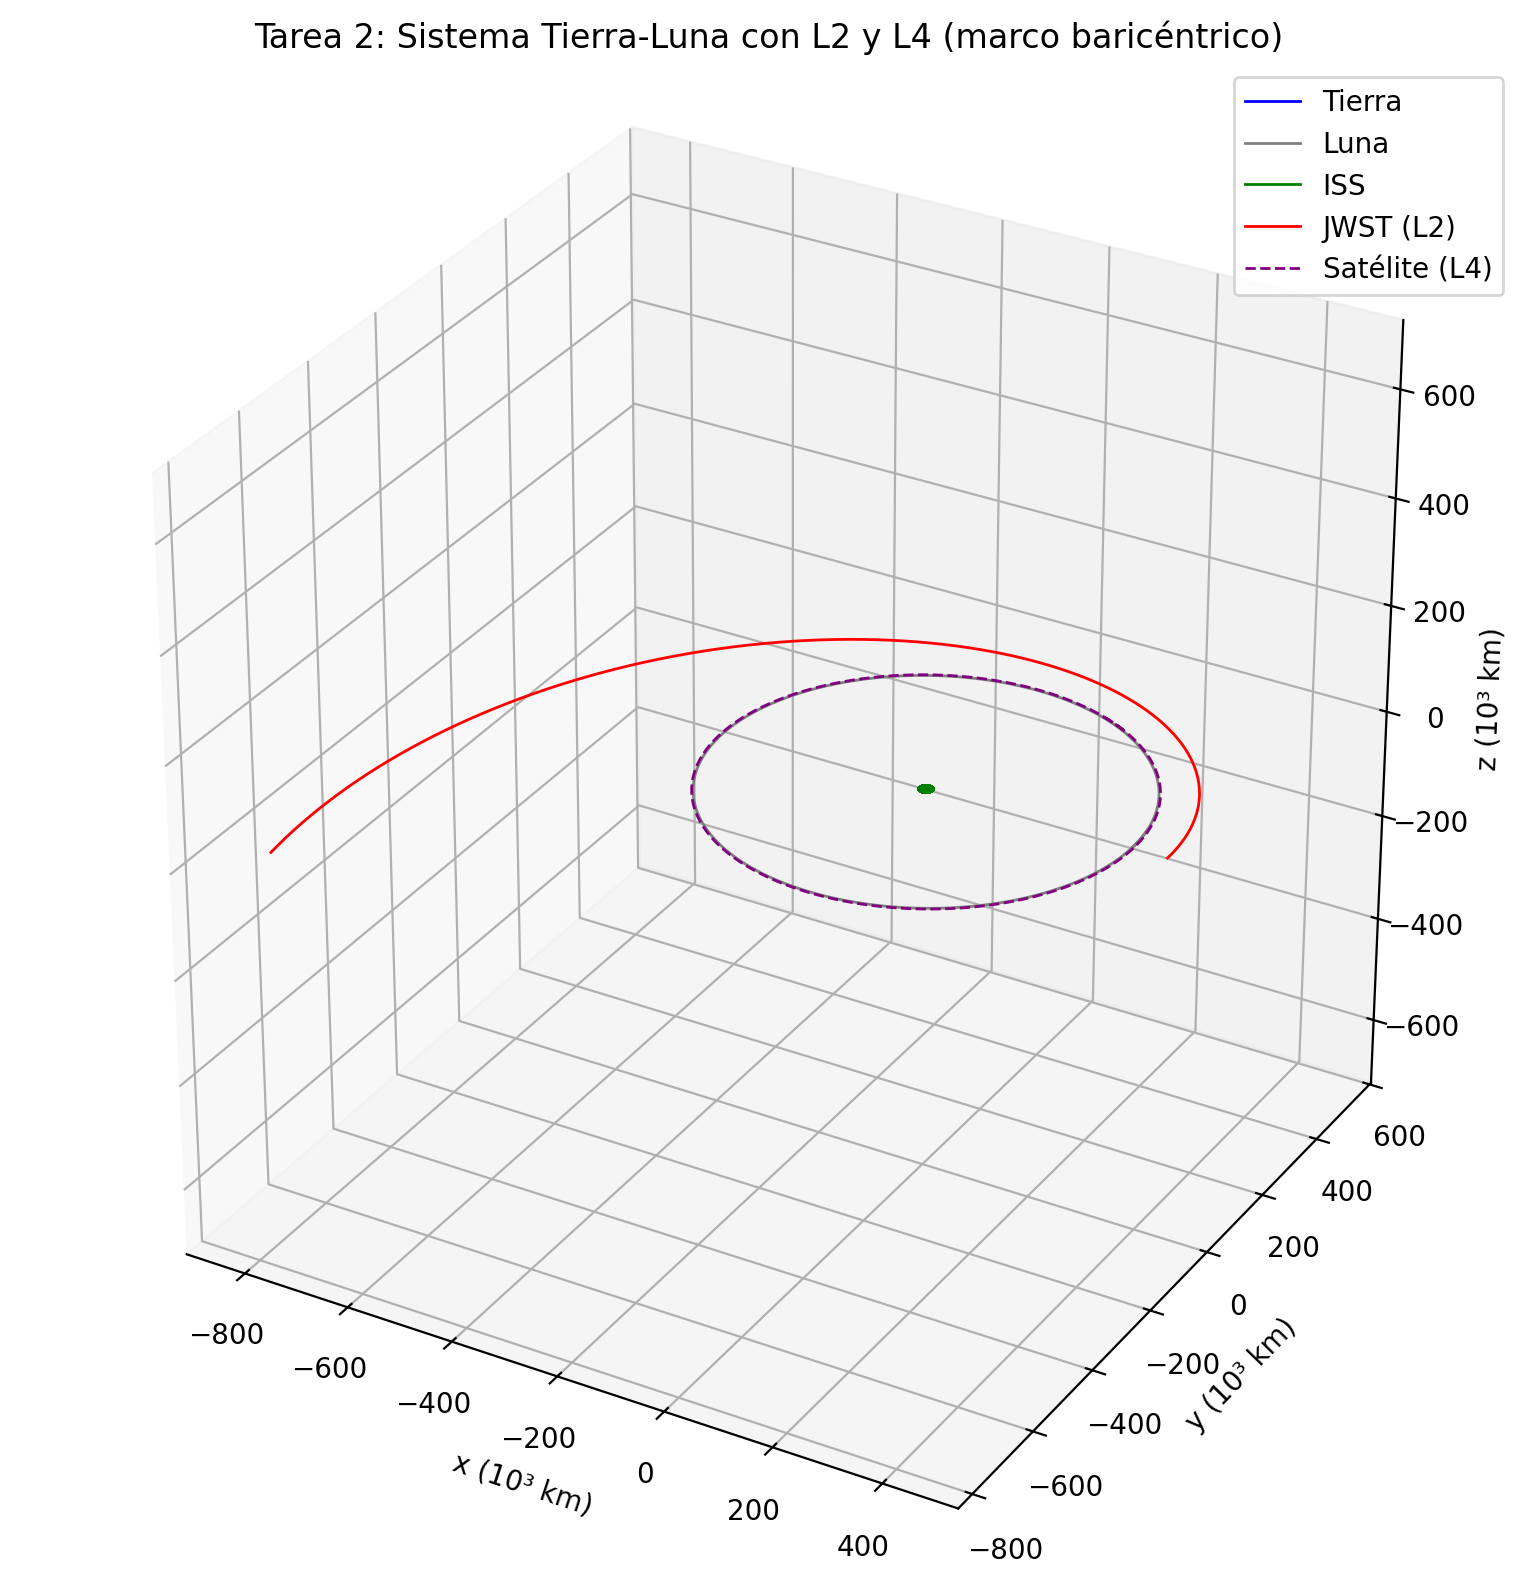
\includegraphics[width=0.6\textwidth]{T2v2_01_Sistema_3D.png}
	\caption{Tarea 2: trayectorias del sistema de 5 cuerpos en el marco baricéntrico.}
	\label{fig:t2_3d}
\end{figure}

\begin{figure}[H]
	\centering
	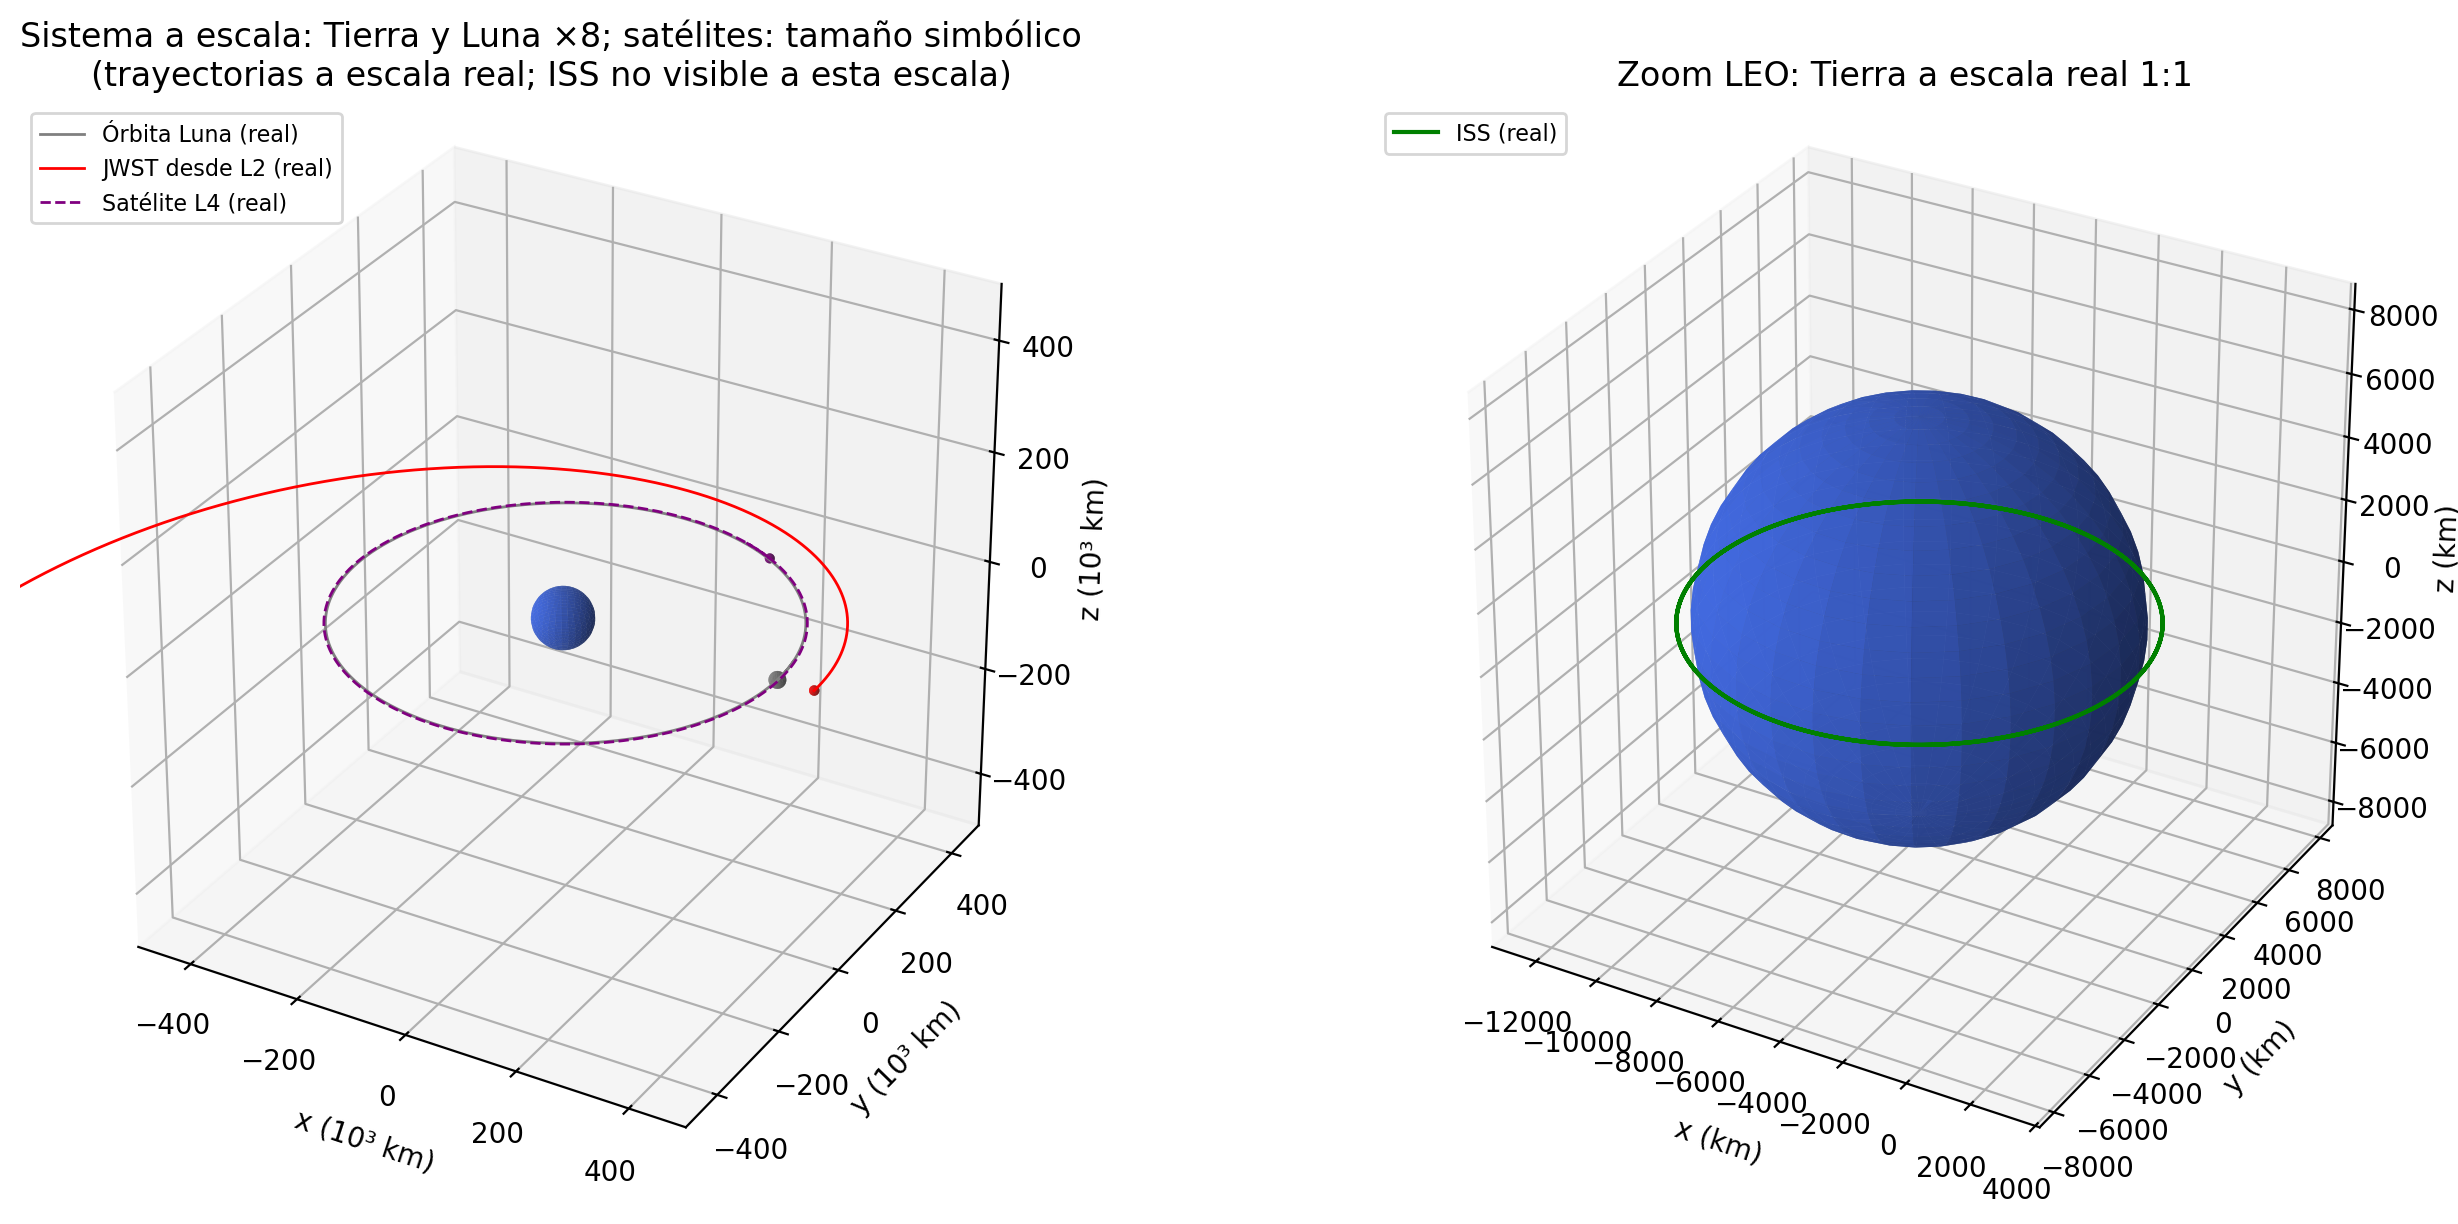
\includegraphics[width=0.98\textwidth]{T2v2_04_Sistema_Escalado.png}
	\caption{Tarea 2: escala del sistema. Izquierda: Tierra y Luna magnificadas $\times 8$ y satélites con tamaño simbólico (las trayectorias Luna-JWST-$L_4$ están a escala real; a esta escala la órbita de la ISS es más pequeña que el grosor de la esfera terrestre). Derecha: zoom a LEO con la Tierra a escala real $1{:}1$ y la órbita de la ISS.}
	\label{fig:t2_escala}
\end{figure}

\begin{figure}[H]
	\centering
	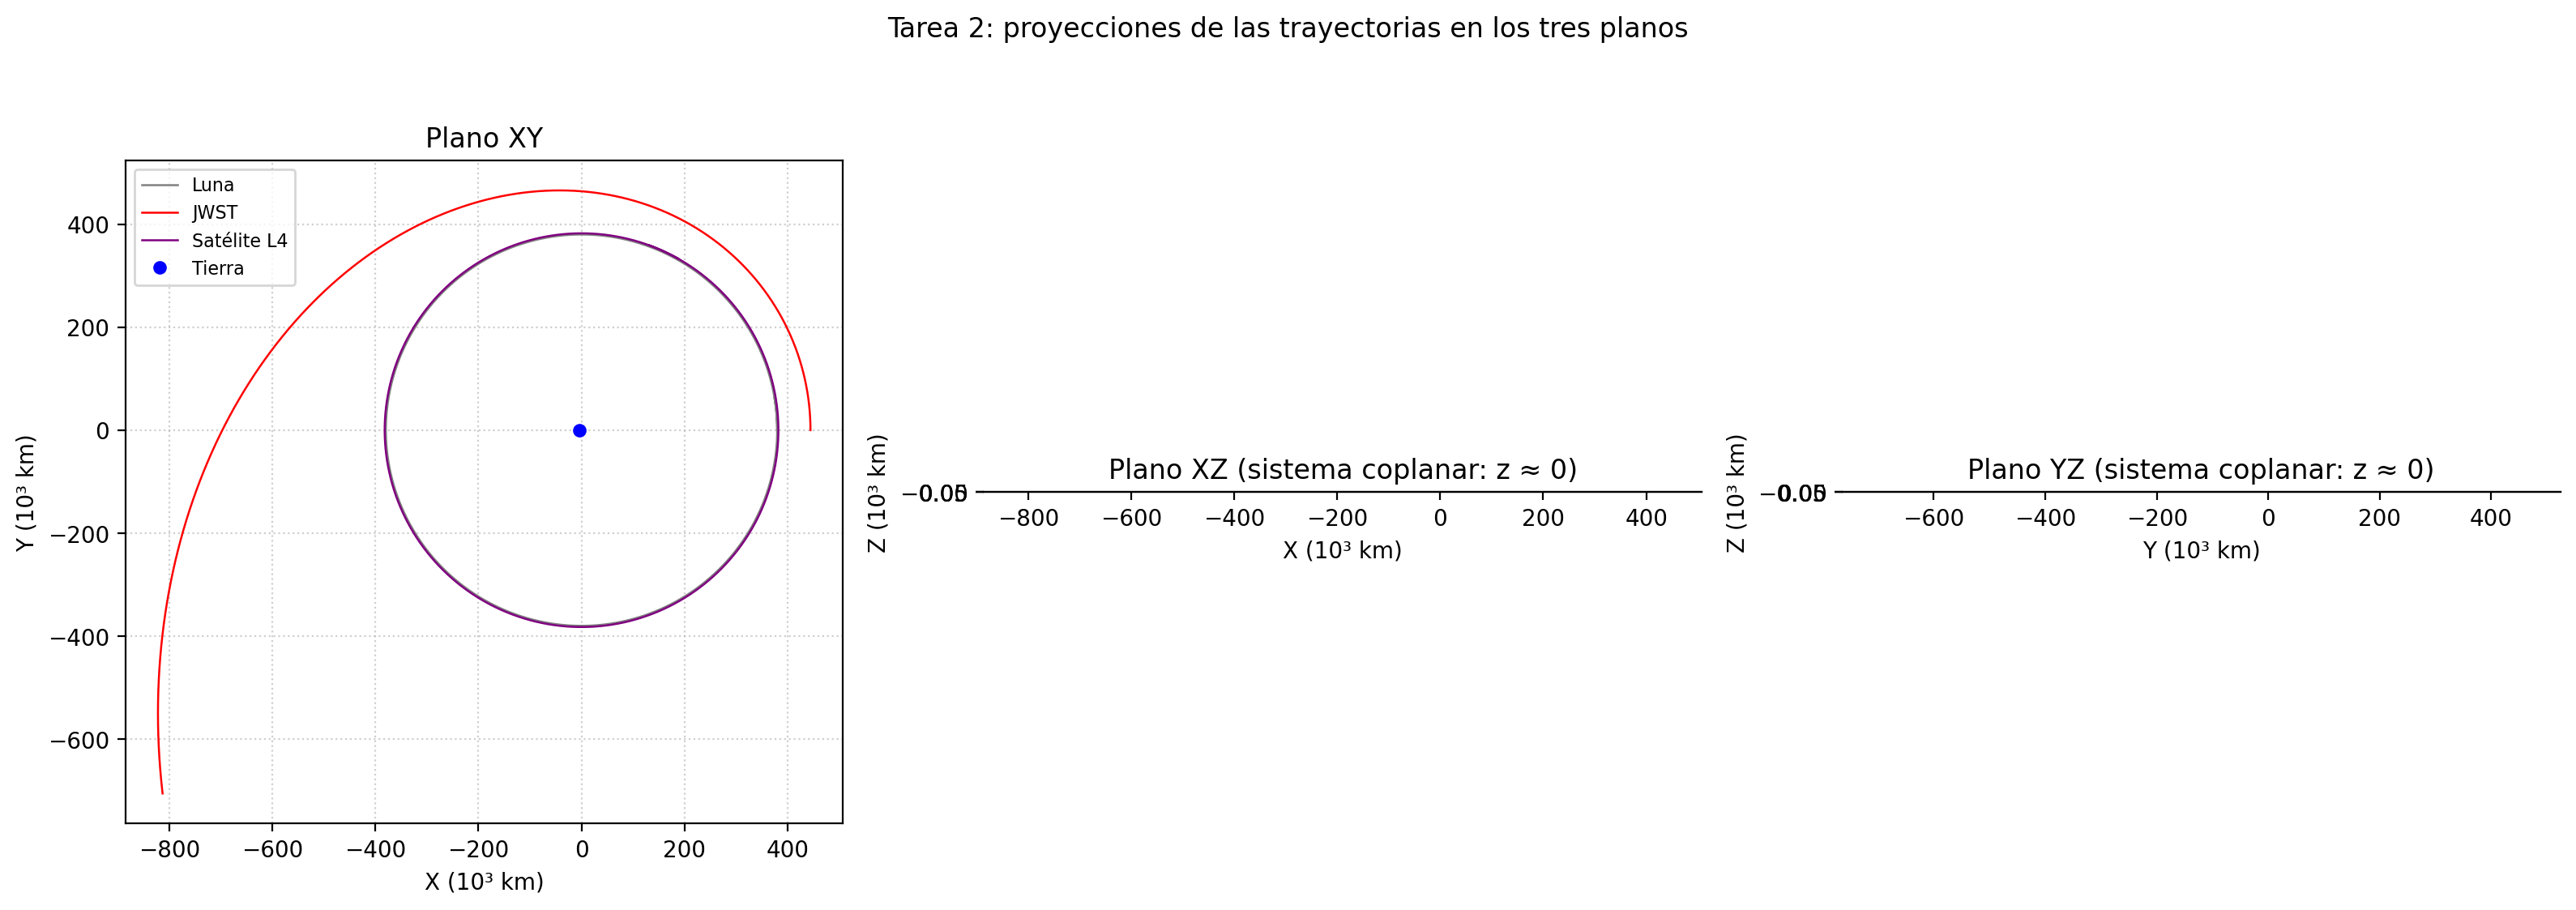
\includegraphics[width=0.98\textwidth]{T2v2_05_Planos.png}
	\caption{Tarea 2: proyecciones de las trayectorias sobre los tres planos. El sistema es coplanar por construcción (condiciones iniciales con $z = 0$), por lo que las proyecciones XZ e YZ colapsan a segmentos: el movimiento vertical es nulo.}
	\label{fig:t2_planos}
\end{figure}

\subsubsection{Localización numérica de los cinco puntos de Lagrange}
\label{sec:lagrange}
Los puntos de Lagrange se calculan en el formalismo del problema circular restringido de
tres cuerpos (CR3BP). En el marco que rota con las primarias, con unidades normalizadas
(separación $=1$, masa total $=1$, parámetro de masa $\mu = M_L/(M_T+M_L) = 0.01214$,
Tierra en $(-\mu, 0)$ y Luna en $(1-\mu, 0)$), el potencial efectivo es
\begin{equation}
	\Omega(x, y) = \frac{1}{2}\left(x^2 + y^2\right) + \frac{1-\mu}{r_1} + \frac{\mu}{r_2},
	\qquad r_k = \left\|\mathbf{r} - \mathbf{r}_k\right\|
\end{equation}
y los puntos de equilibrio son sus \textbf{puntos críticos}. Los colineales
$L_1, L_2, L_3$ (sobre el eje de las primarias) satisfacen
\begin{equation}
	\frac{\partial \Omega}{\partial x} = x - (1-\mu)\frac{x+\mu}{|x+\mu|^3} - \mu\,\frac{x-1+\mu}{|x-1+\mu|^3} = 0,
	\label{eq:domega}
\end{equation}
ecuación trascendente que se resuelve con la \textbf{rutina de bisección} de la Fase II,
sembrada en intervalos con cambio de signo garantizado: $L_1$ entre las primarias,
$L_2$ más allá de la Luna y $L_3$ al lado opuesto de la Tierra. Los triangulares son
solución exacta:
\begin{equation}
	L_{4,5} = \left(\tfrac{1}{2} - \mu,\; \pm\tfrac{\sqrt{3}}{2}\right),
\end{equation}
vértices del triángulo equilátero, estables siempre que $\mu < \mu_{\text{Routh}} =
\tfrac{1}{2}\left(1 - \tfrac{\sqrt{69}}{9}\right) \approx 0.0385$ (cumplido con:
$\mu = 0.0121$). Resultados numéricos:

\begin{table}[H]
	\centering
	\begin{tabular}{lrrl}
		\toprule
		Punto & Distancia a la Tierra (km) & Distancia a la Luna (km) & Método \\
		\midrule
		$L_1$ & $326\,390$ & $58\,010$  & bisección de la Ec.~(\ref{eq:domega}) \\
		$L_2$ & $448\,904$ & $64\,504$  & bisección de la Ec.~(\ref{eq:domega}) \\
		$L_3$ & $381\,677$ & $766\,077$ & bisección de la Ec.~(\ref{eq:domega}) \\
		$L_4$ & $384\,400$ & $384\,400$ & triángulo equilátero (exacto) \\
		$L_5$ & $384\,400$ & $384\,400$ & triángulo equilátero (exacto) \\
		\bottomrule
	\end{tabular}
	\caption{Los cinco puntos de Lagrange del sistema Tierra-Luna calculados por el módulo \texttt{puntos\_lagrange\_CR3BP}.}
	\label{tab:lagrange}
\end{table}

\begin{figure}[H]
	\centering
	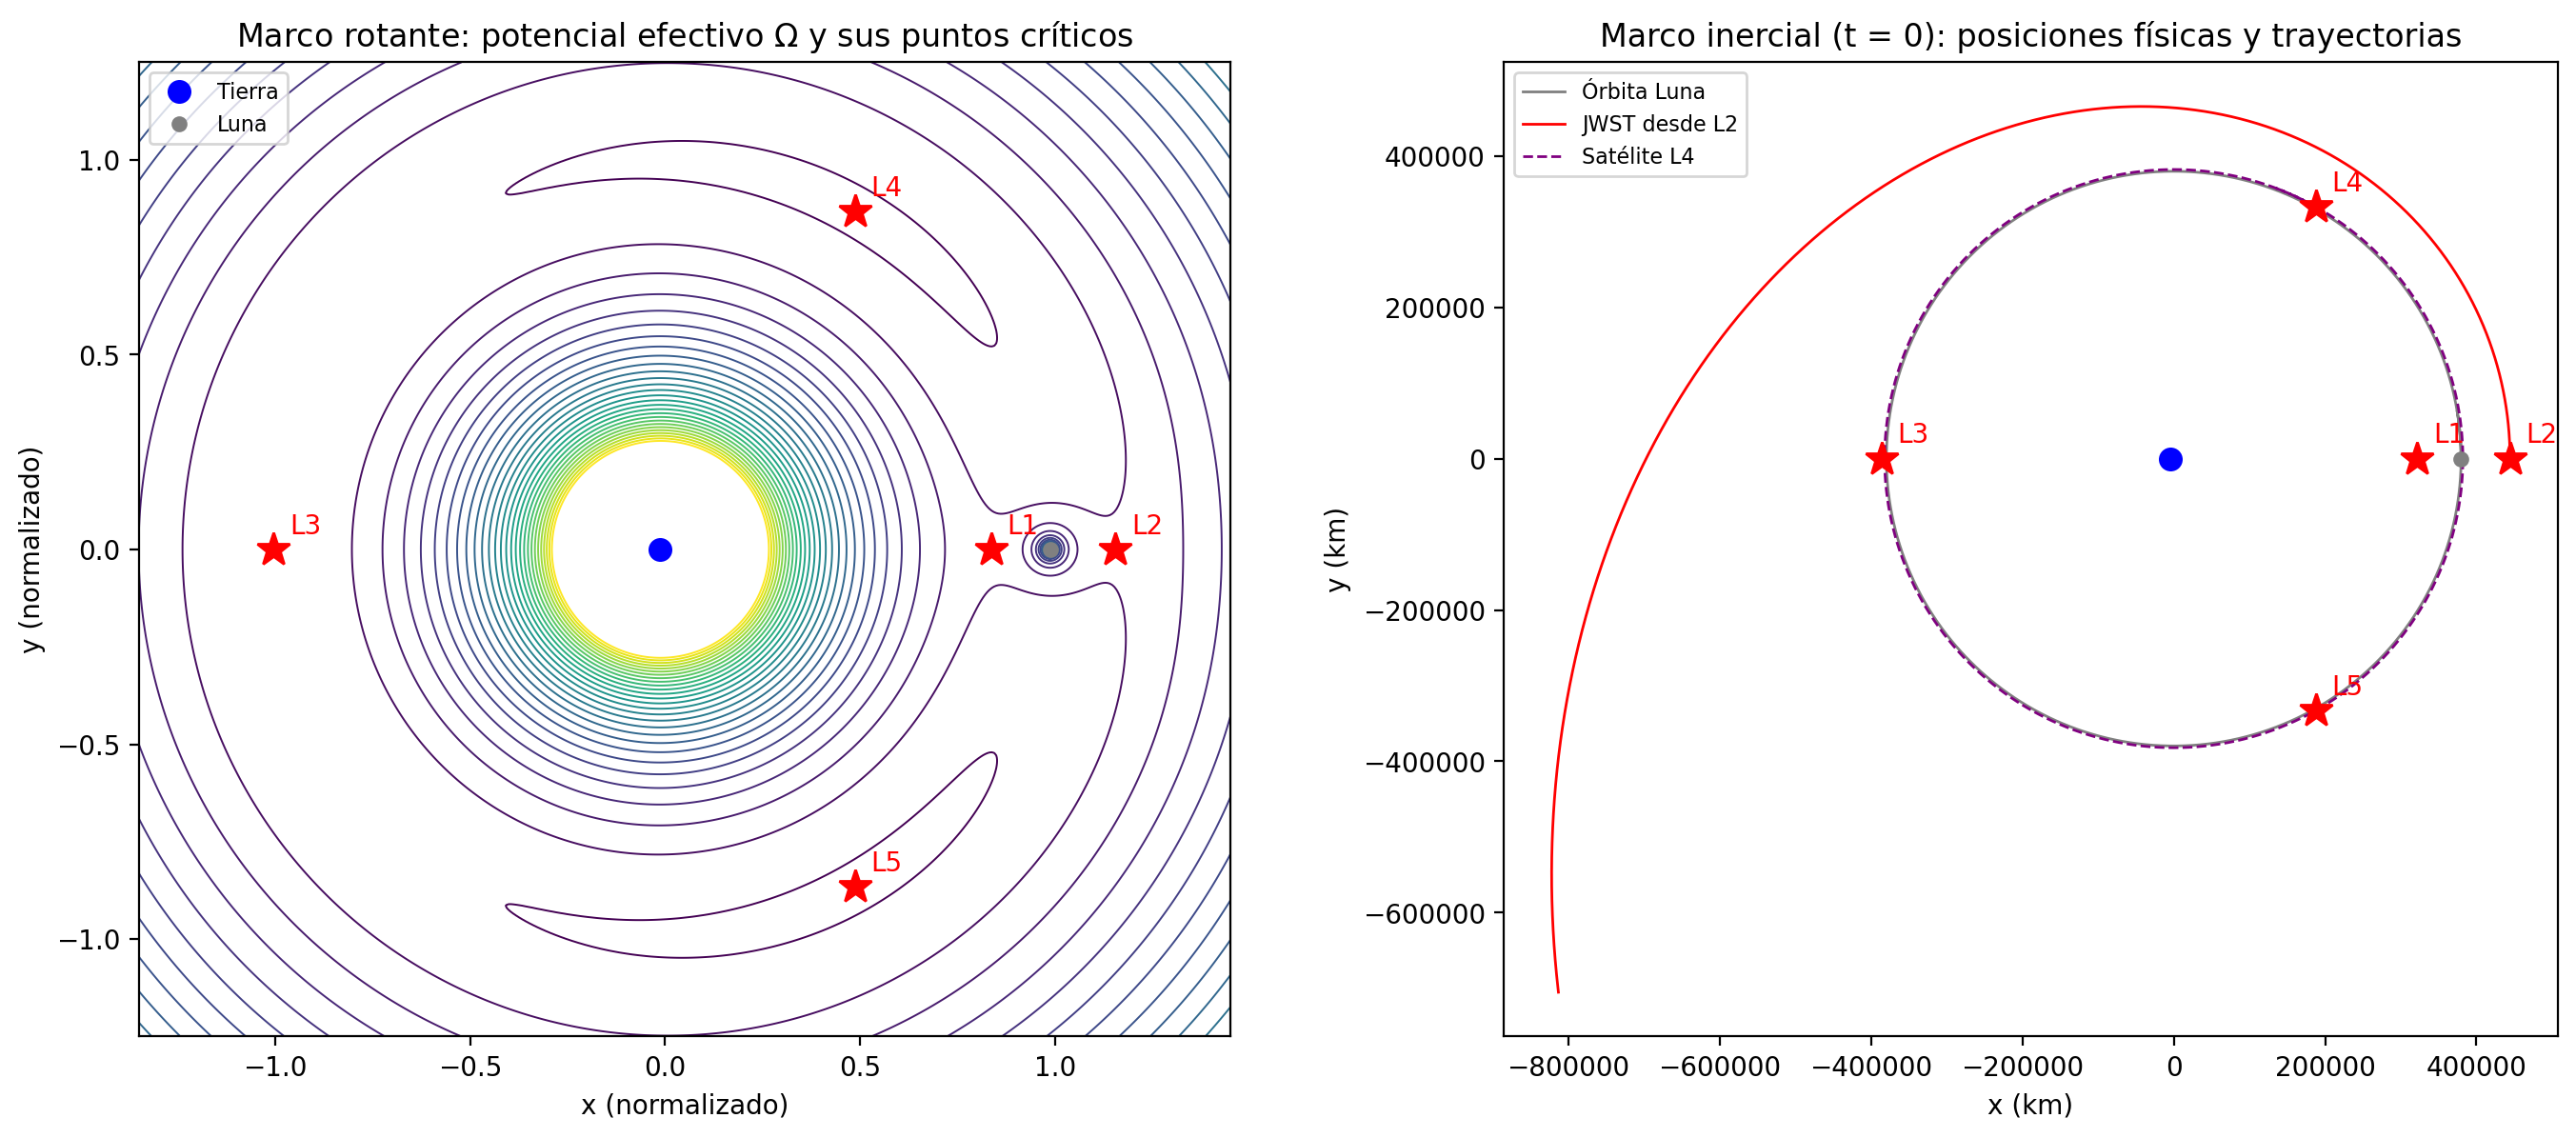
\includegraphics[width=0.98\textwidth]{T2v2_06_Puntos_Lagrange.png}
	\caption{Tarea 2: los cinco puntos de Lagrange. Izquierda: contornos del potencial efectivo $\Omega$ en el marco rotante (unidades normalizadas); los puntos colineales son puntos de silla de esta superficie y $L_4/L_5$ sus máximos. Derecha: posiciones físicas en el marco inercial en $t = 0$, superpuestas a las trayectorias simuladas: el satélite de prueba liba alrededor de $L_4$ mientras el JWST parte de $L_2$ y diverge.}
	\label{fig:t2_lagrange}
\end{figure}

\begin{figure}[H]
	\centering
	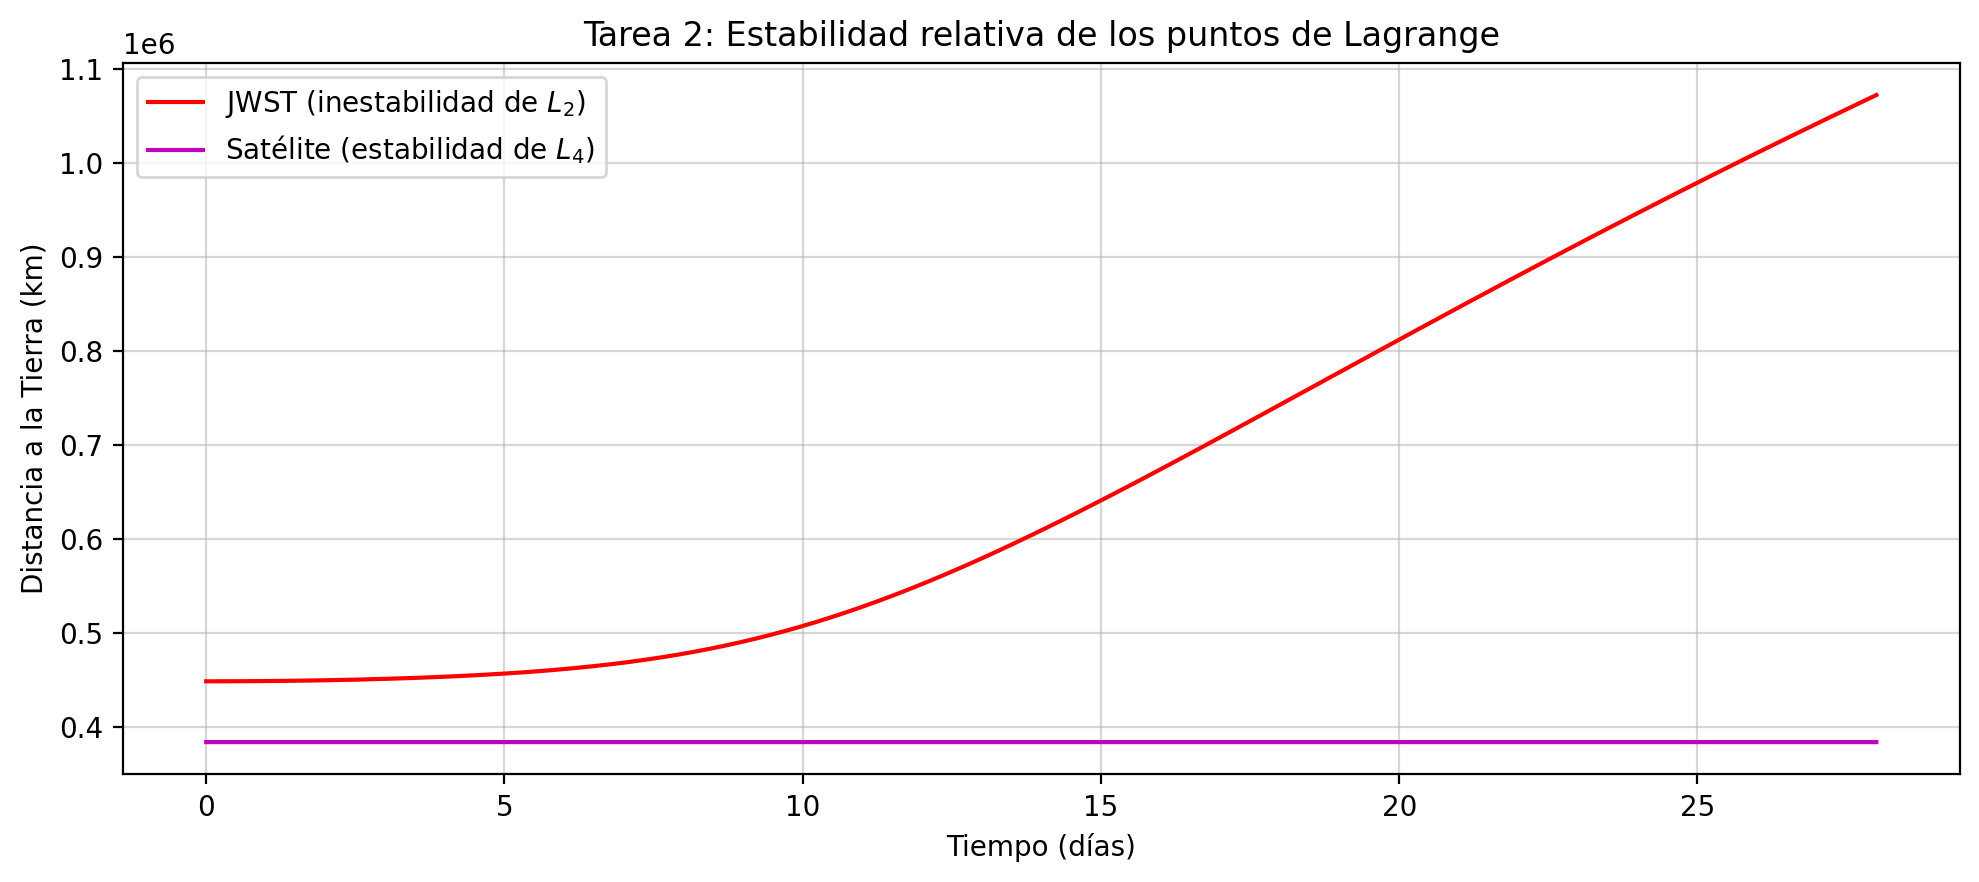
\includegraphics[width=0.85\textwidth]{T2v2_02_Distancias.png}
	\caption{Tarea 2: contraste de estabilidad. El satélite en $L_4$ (triángulo equilátero, punto de equilibrio estable para $\mu < 0.0385$; aquí $\mu = 0.0121$) permanece libando alrededor de su posición nominal, mientras el satélite en $L_2$ (punto de silla) diverge exponencialmente en pocos días.}
	\label{fig:t2_distancias}
\end{figure}

El análisis cuantitativo confirma la teoría del potencial efectivo co-rotante: $L_4$ es un \textbf{mínimo} del potencial efectivo (estabilidad condicionada al criterio de Routh, satisfecho por el sistema Tierra-Luna con margen), mientras que $L_1$--$L_3$ son \textbf{puntos de silla}: cualquier perturbación numérica infinitesimal ---como el error de truncamiento del propio RK4--- crece exponencialmente, reproduciendo el comportamiento real que obliga a misiones como JWST a ejecutar maniobras de \textit{station-keeping}.

\subsection{Tarea 3: Expansión $N$-Cuerpos (Sistema Solar Interior en 3D)}

Sistema de \textbf{8 cuerpos}: Sol, Mercurio, Venus, Tierra, Luna, Marte, Fobos y Deimos, con duración de 730 días e integrador simpléctico. Las condiciones iniciales son: Mercurio desde sus elementos orbitales medios ($a = 57.9\times10^6$ km, $e = 0.2056$, $i = 7.0^\circ$, $\Omega = 48.33^\circ$, $\omega = 29.124^\circ$, $M_0 = 0$) transformados con el módulo de la Sección~\ref{sec:kepler_solver}; los demás planetas en órbitas coplanares circulares con velocidades vis-viva ($v = \sqrt{\mu_\odot/r}$); las lunas con velocidades circulares relativas a sus planetas. Son condiciones simplificadas de tipo pedagógico, no efemérides.

El paso se fija en $h = 600$ s (justificación cuantitativa en la Fase IV): el cuerpo más exigente no es Mercurio sino Fobos (período orbital $7.65$ h), que exige $\gtrsim 40$ muestras por órbita.

\begin{figure}[H]
	\centering
	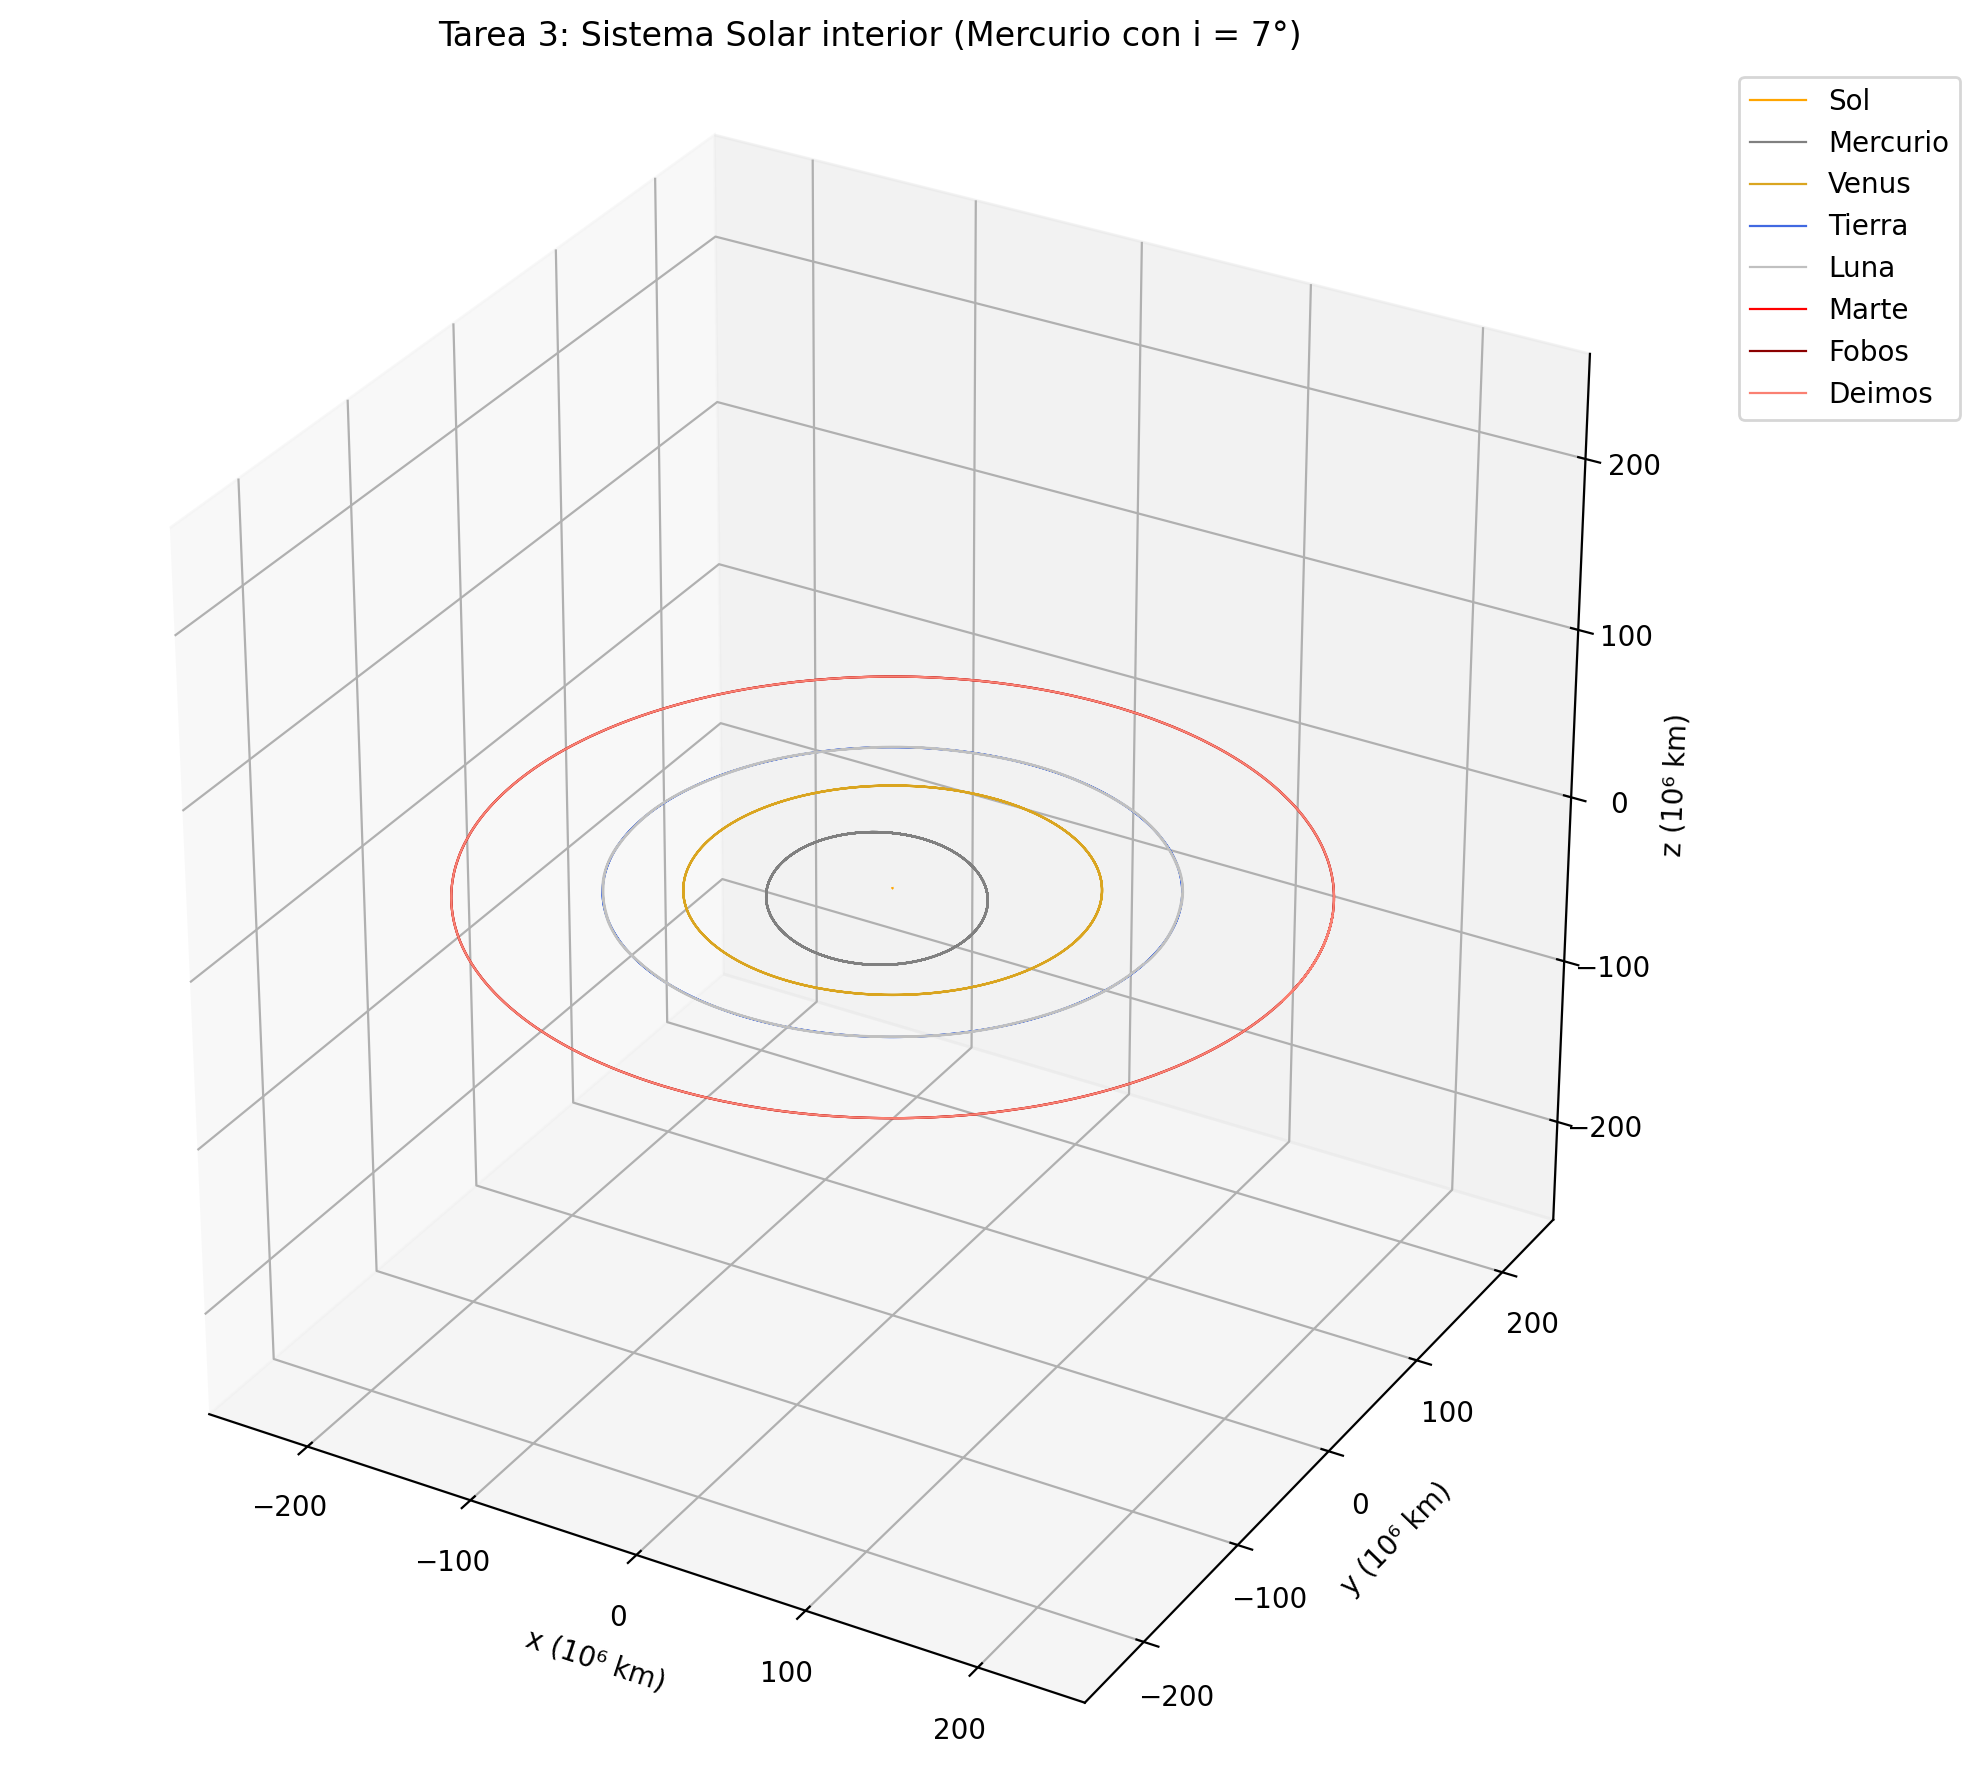
\includegraphics[width=0.72\textwidth]{T3v2_01_Sistema_3D.png}
	\caption{Tarea 3: sistema solar interior en 3D con relación de aspecto $1{:}1{:}1$. La órbita de Mercurio emerge del plano de la eclíptica por su inclinación de $7^\circ$.}
	\label{fig:t3_3d}
\end{figure}

\begin{figure}[H]
	\centering
	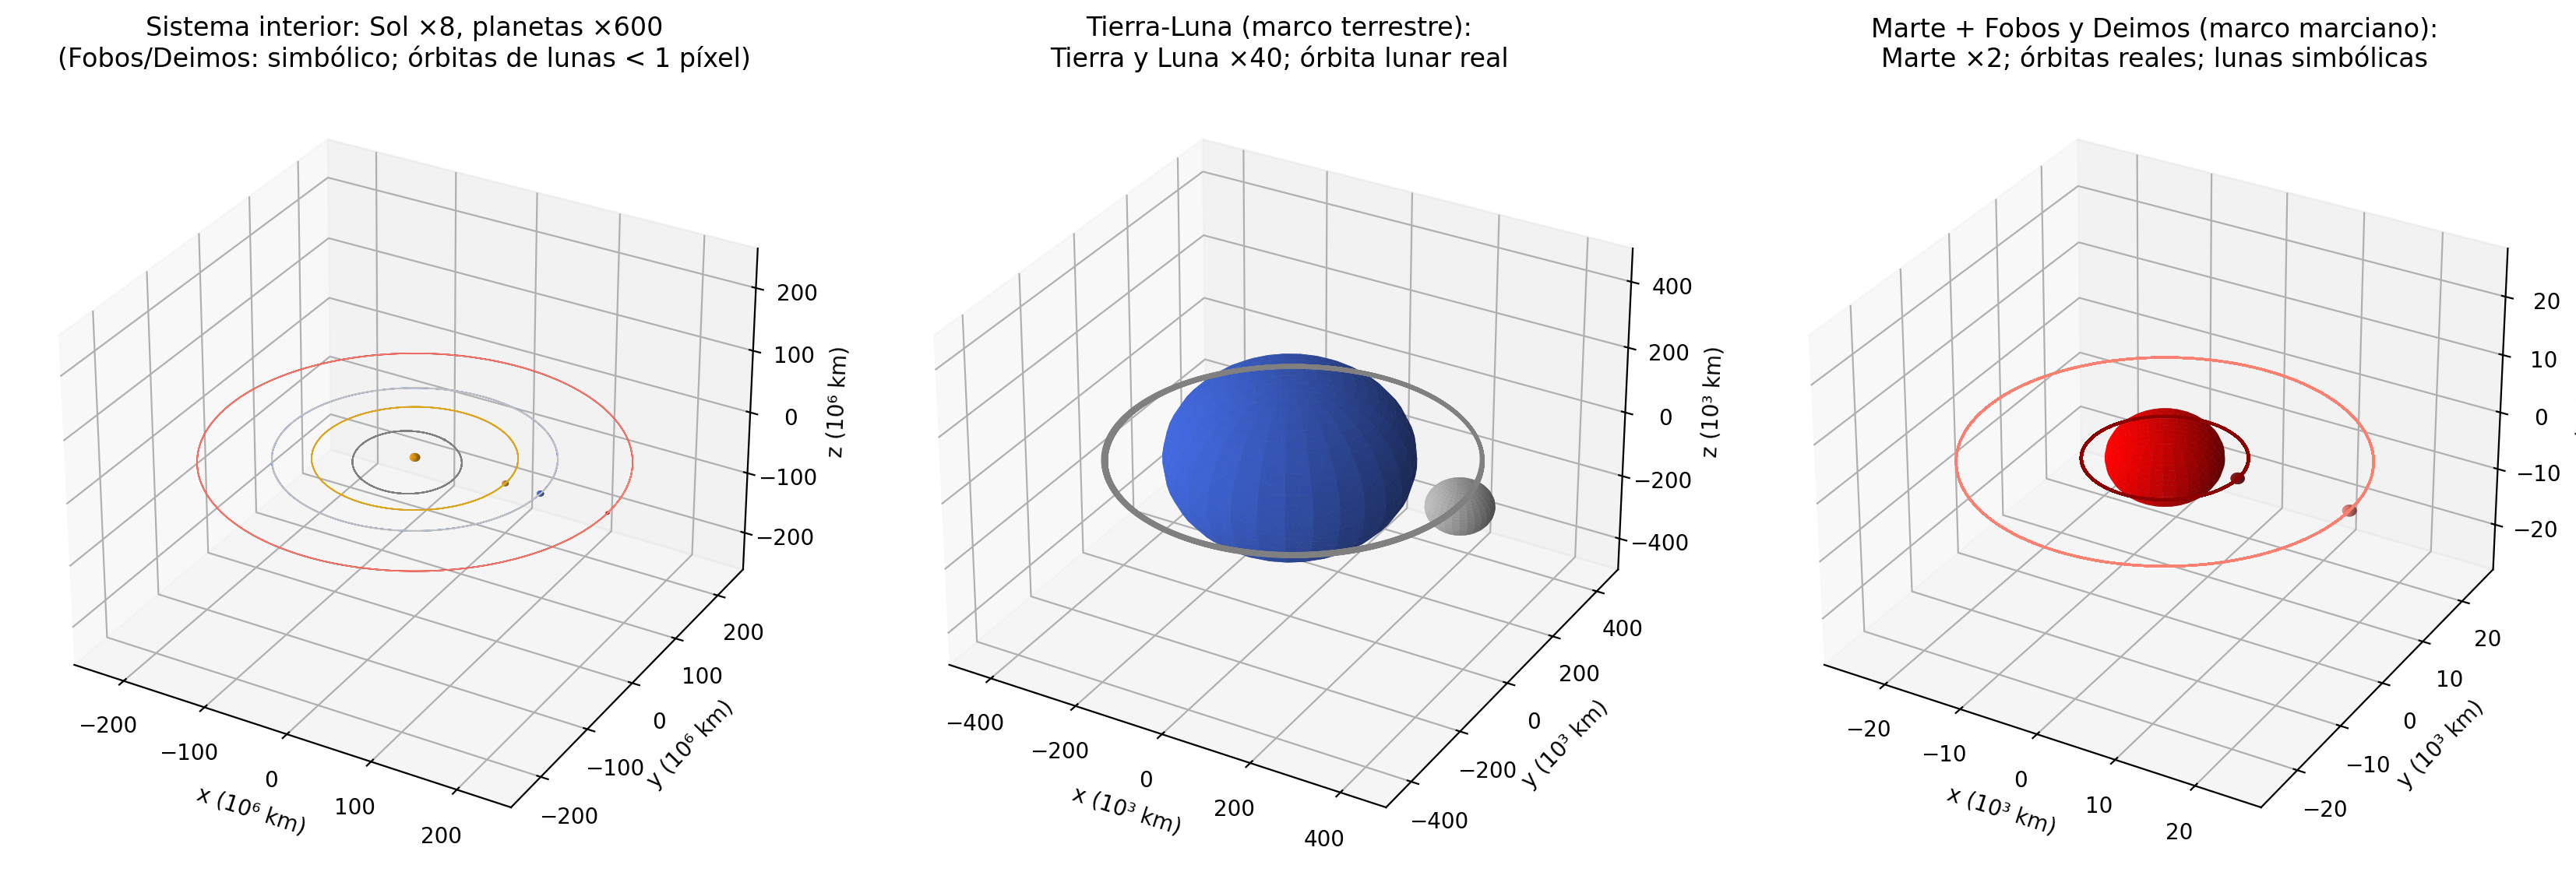
\includegraphics[width=0.98\textwidth]{T3v2_05_Escala_Cuerpos.png}
	\caption{Tarea 3: escalas por subsistema. Izquierda: sistema interior con Sol $\times 8$ y planetas $\times 600$ (las órbitas de las lunas son menores que un píxel a esta escala). Centro: subsistema Tierra-Luna en el marco terrestre, con Tierra y Luna $\times 40$ y la órbita lunar real. Derecha: subsistema marciano con Marte $\times 2$, órbitas reales de Fobos y Deimos y lunas con tamaño simbólico. En todos los casos las trayectorias están a escala real y solo el tamaño de las esferas está magnificado por el factor indicado.}
	\label{fig:t3_escala}
\end{figure}

\begin{figure}[H]
	\centering
	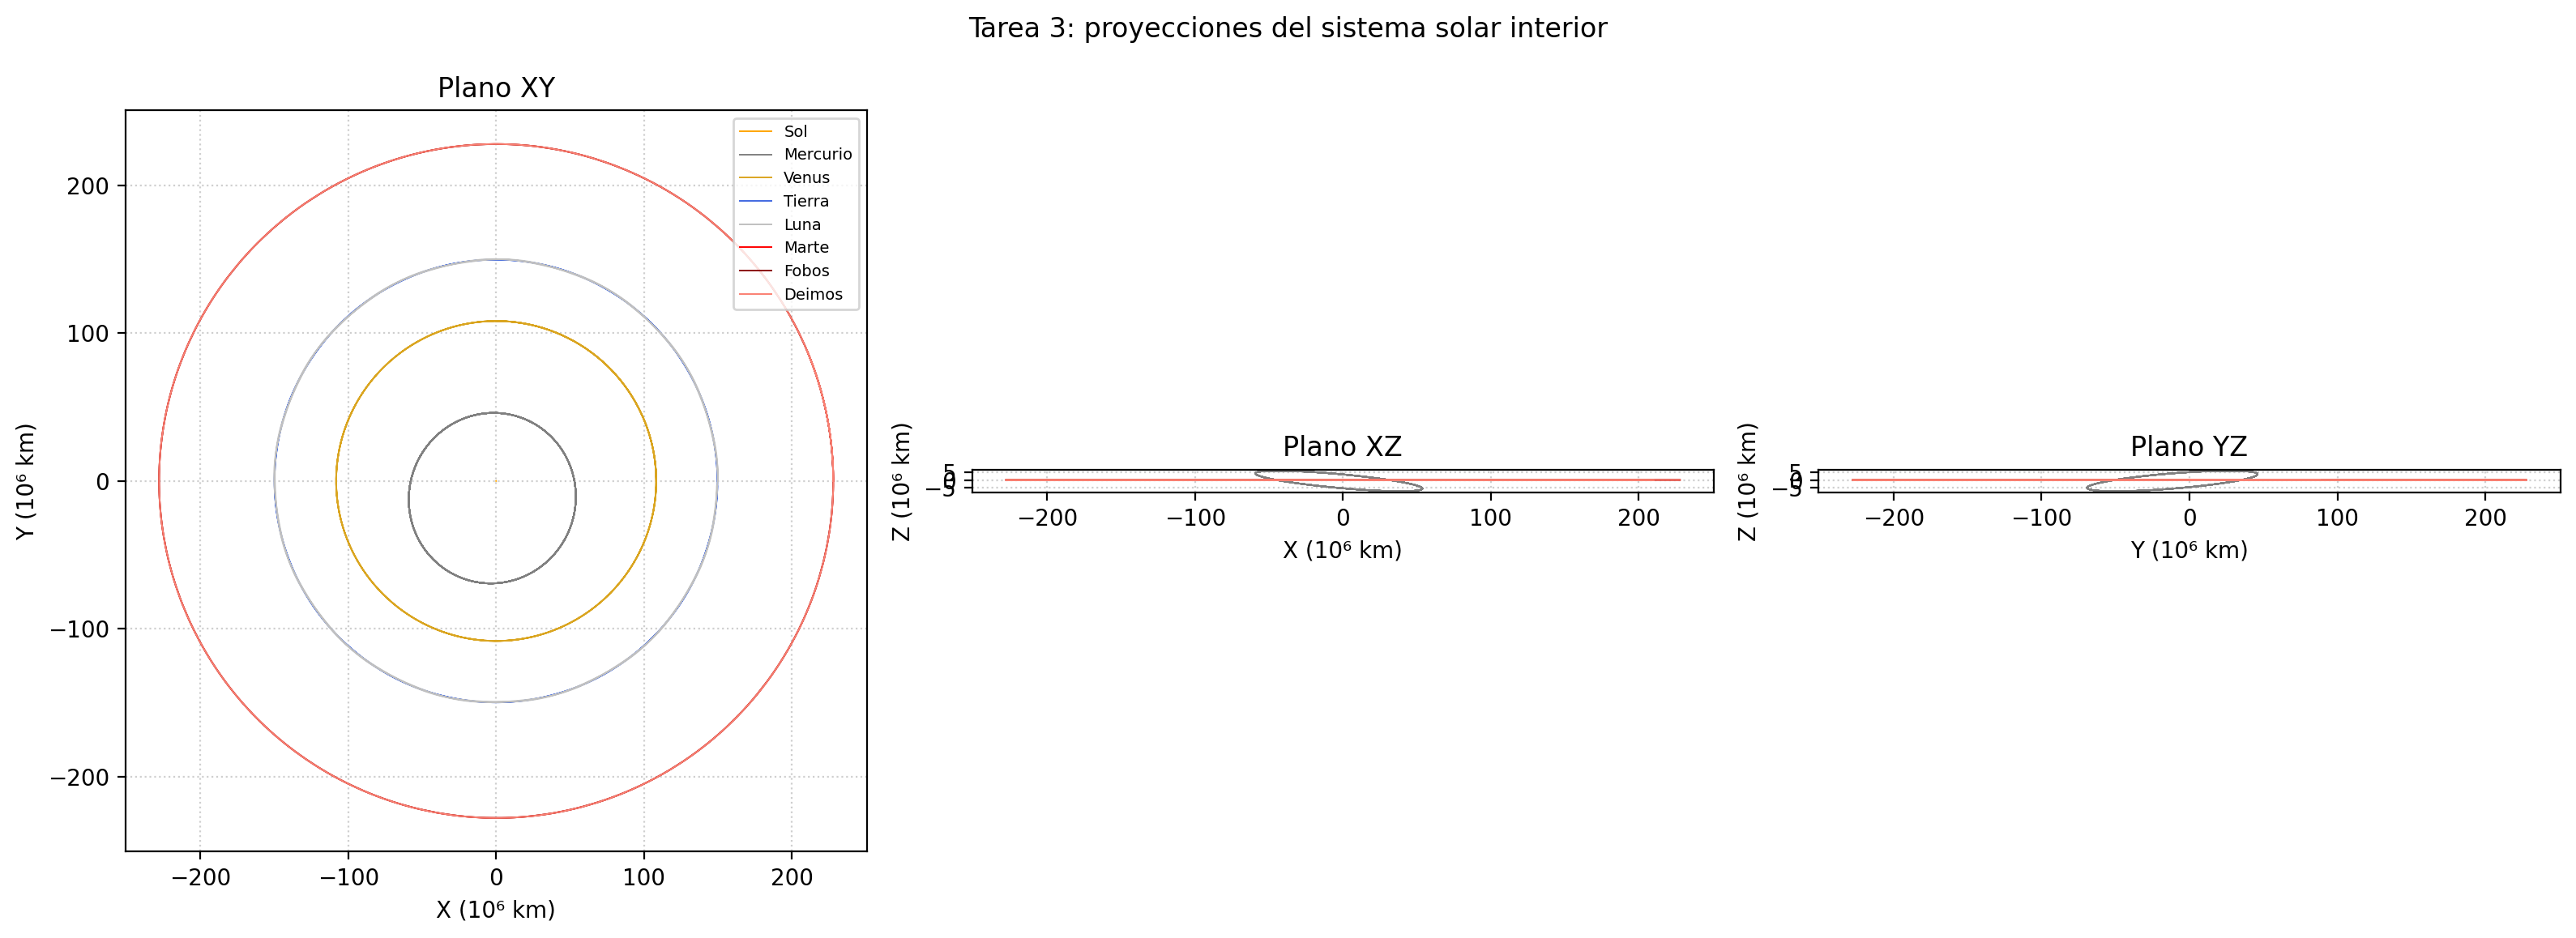
\includegraphics[width=0.98\textwidth]{T3v2_06_Planos.png}
	\caption{Tarea 3: proyecciones del sistema solar interior sobre los tres planos. En el plano XY (eclíptica) las órbitas son casi concéntricas; en XZ e YZ solo Mercurio alcanza elevación apreciable ($i = 7^\circ$), visualizando directamente la estructura no coplanar del sistema.}
	\label{fig:t3_planos}
\end{figure}

\begin{figure}[H]
	\centering
	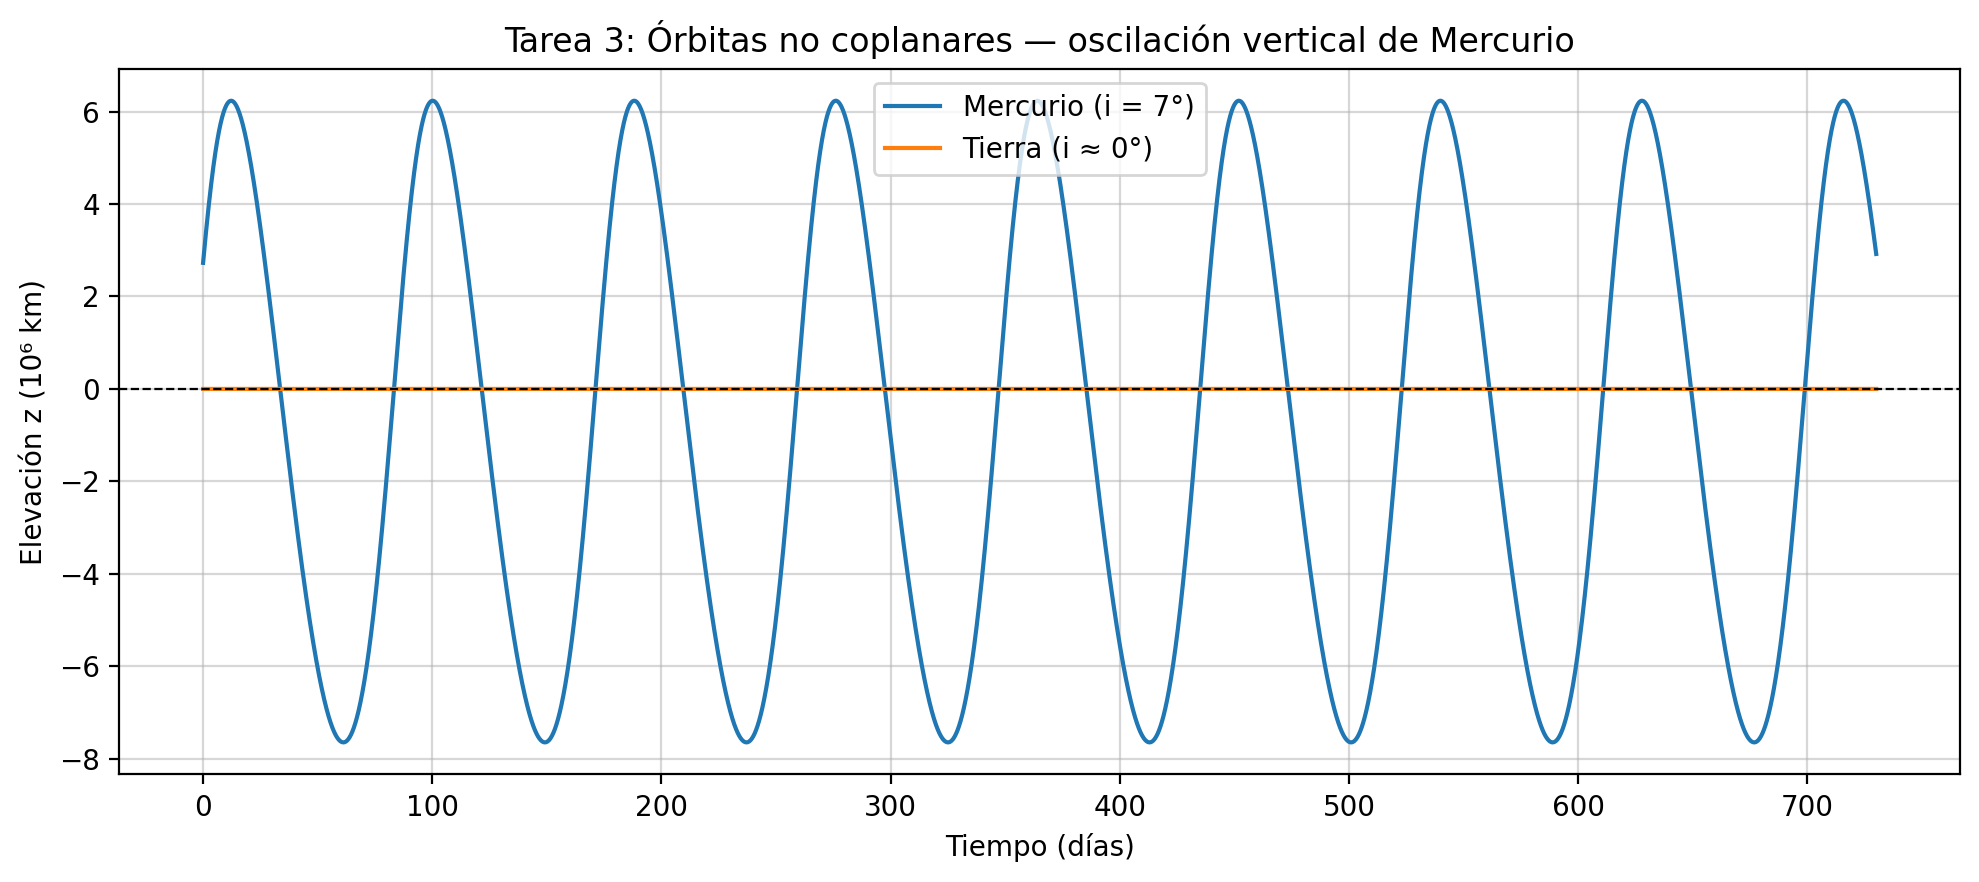
\includegraphics[width=0.85\textwidth]{T3v2_02_Inclinacion_Z.png}
	\caption{Tarea 3: oscilación vertical de Mercurio ($i = 7^\circ$) frente a la Tierra ($i \approx 0^\circ$): visualización directa de las órbitas no coplanares.}
	\label{fig:t3_z}
\end{figure}

\subsubsection{Análisis de precesión orbital 3D (requisito de la Tarea 3)}
A partir del registro de estados se calculan los \textbf{elementos osculantes} de Mercurio respecto al Sol en cada paso. La regresión por mínimos cuadrados de la longitud del perihelio $\varpi = \Omega + \omega$ y de la longitud del nodo $\Omega$ da:
\begin{align}
	\dot\varpi_{\text{3D}} &= +148.7''/\text{siglo} & \dot\Omega_{\text{3D}} &= -471.3''/\text{siglo}
\end{align}
Estos valores son la \textbf{precesión secular newtoniana} producada por las perturbaciones de los planetas interiores del modelo. Como referencia, la precesión newtoniana total de Mercurio (todos los planetas) es $\approx 532''$/siglo ---dominada por Júpiter ($\approx 154''$/siglo), ausente de este modelo--- y la corrección relativista es $42.98''$/siglo, no incluida al tratarse de un modelo estrictamente newtoniano. La concordancia de orden de magnitud con la teoría secular clásica valida el análisis.

\subsubsection{Comparación cualitativa 3D vs.\ 2D planar (requisito de la Tarea 3)}
Se repitió la simulación forzando todos los cuerpos al plano de la eclíptica ($i = 0$, incluido Mercurio). Resultados:
\begin{align}
	\dot\varpi_{\text{2D}} &= +976.4''/\text{siglo} & \text{vs.} && \dot\varpi_{\text{3D}} &= +148.7''/\text{siglo}
\end{align}

\begin{figure}[H]
	\centering
	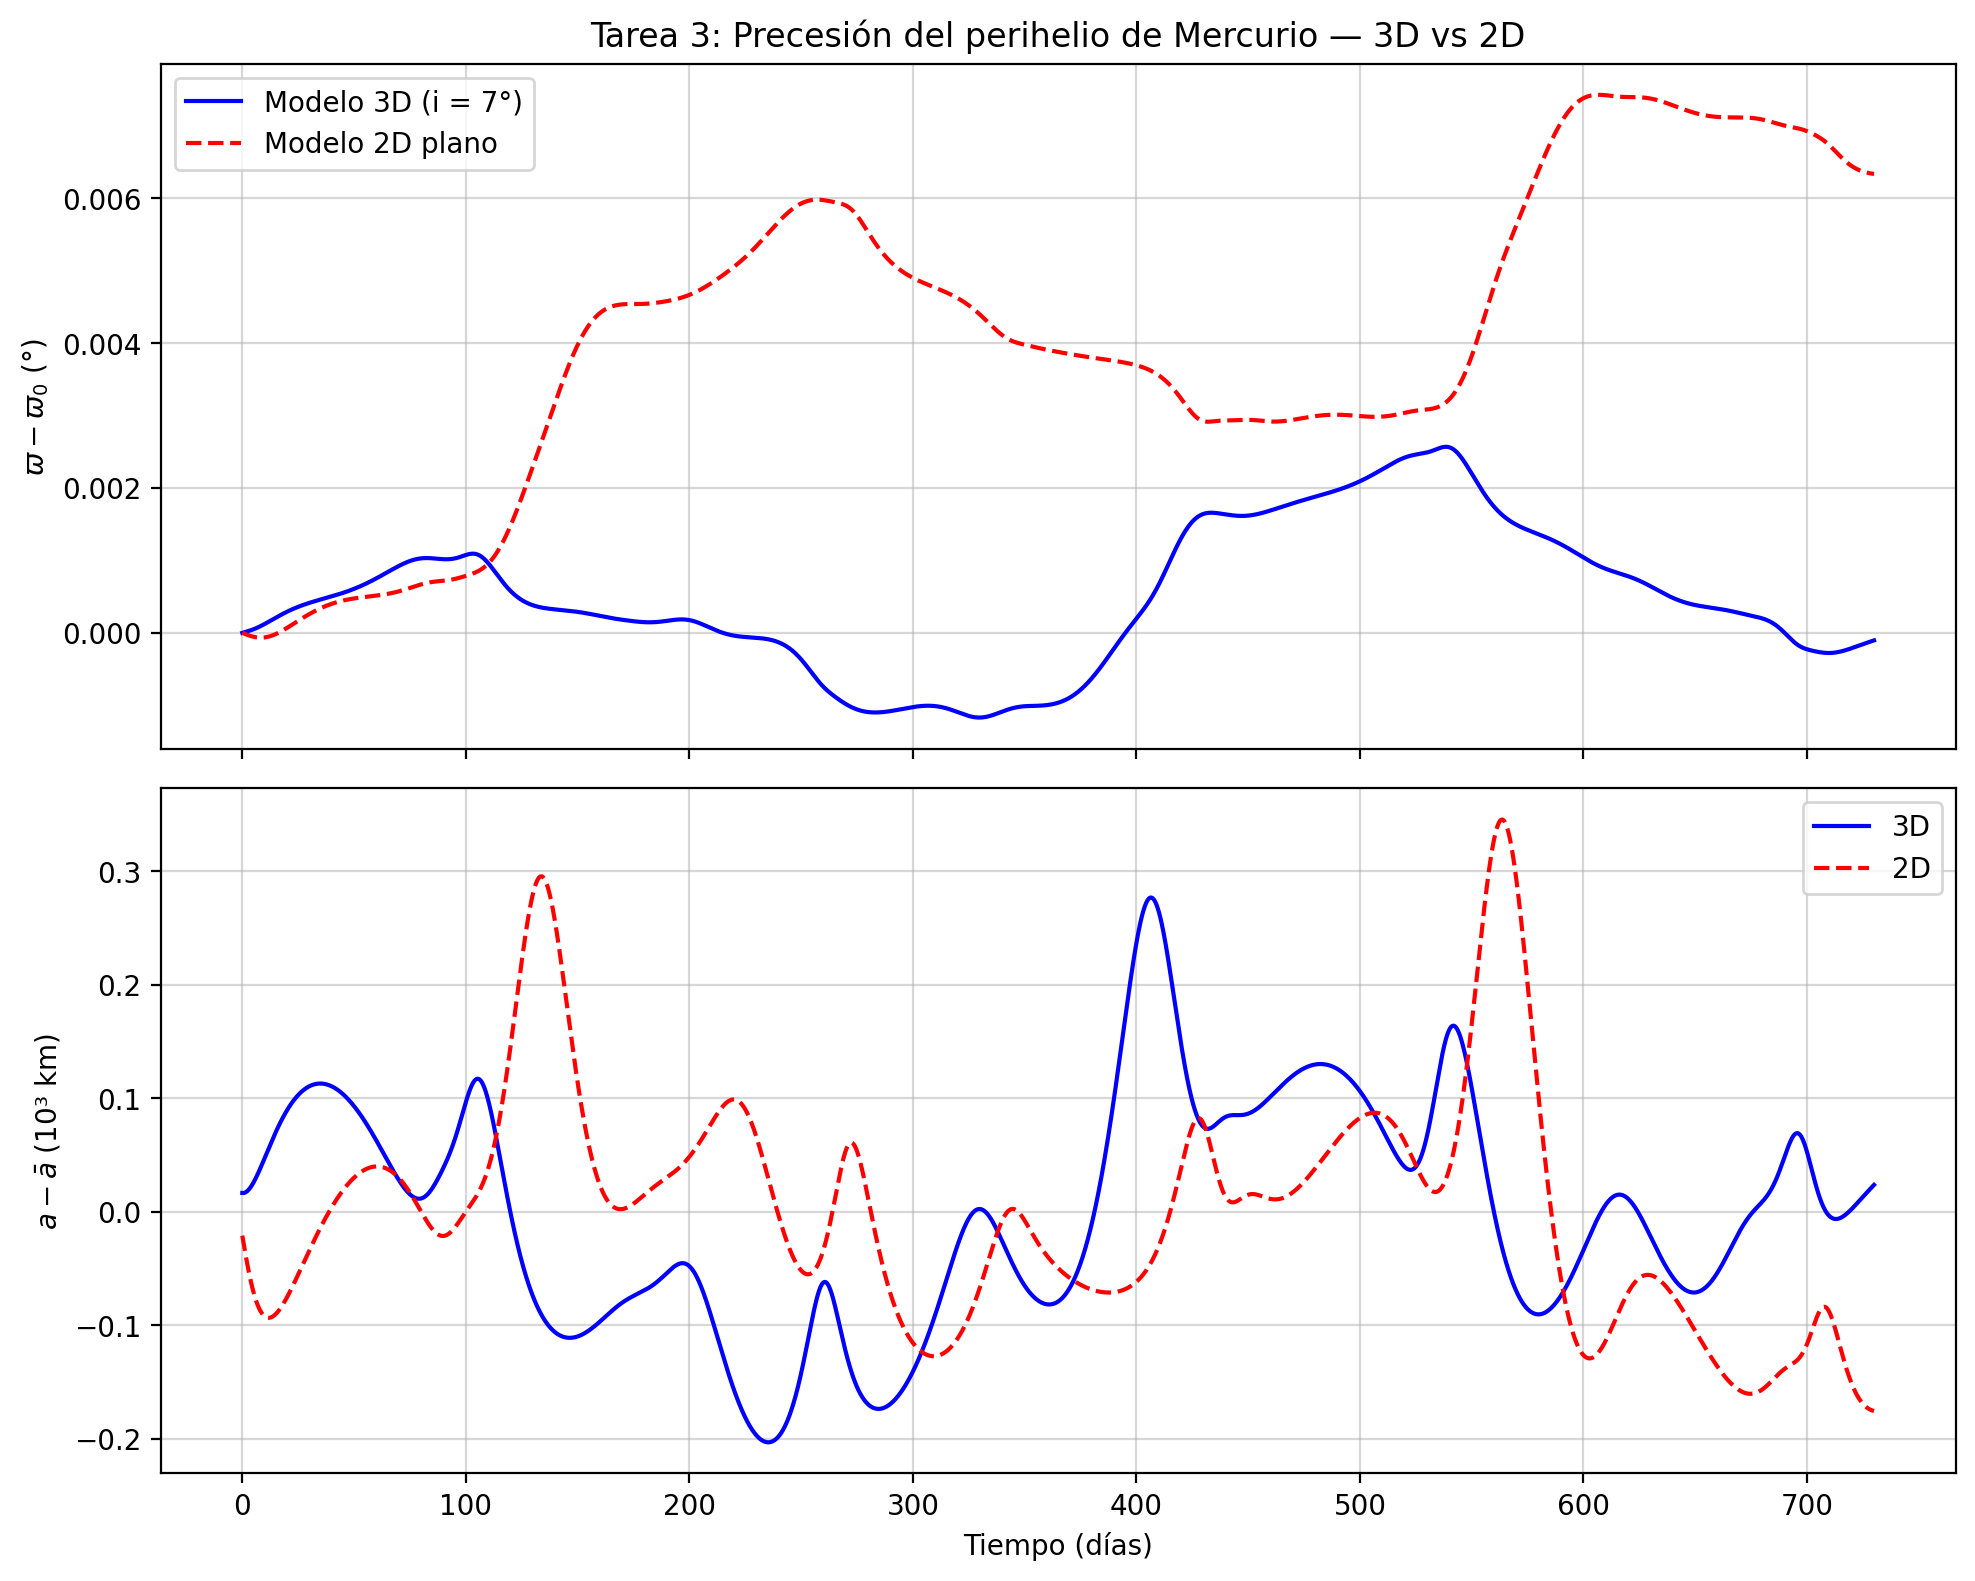
\includegraphics[width=0.9\textwidth]{T3v2_04_Precesion_2Dvs3D.png}
	\caption{Tarea 3: precesión del perihelio de Mercurio en el modelo 3D ($i = 7^\circ$) frente al modelo 2D plano, y oscilación del semieje mayor osculador en ambos modelos.}
	\label{fig:t3_precesion}
\end{figure}

La diferencia es un factor $\sim 6.6$. En el modelo planar todos los momentos angulares planetarios son colineales: la componente de la perturbación perpendicular al plano no existe y toda la pareja perturbadora proyecta sobre la dirección in-plane, inflando la precesión del perihelio. En 3D, parte del torque secular se canaliza en la \textbf{regresión nodal} ($\dot\Omega \neq 0$, medida arriba) y en los modos de inclinación, redistribuyendo la perturbación entre los grados de libertad in-plane y out-of-plane. En cuanto a la estabilidad cualitativa a largo plazo, ambos modelos mantienen el semieje mayor oscilador de Mercurio acotado (oscilaciones de $\sim 10^3$ km), pero el modelo 2D es cualitativamente distinto: no puede representar intercambio inclinación-excentricidad (mecanismo tipo Kozai-Lidov), ni la geometría real de los torques, por lo que \emph{sobreestima} sistemáticamente la precesión y subestima la riqueza dinámica del sistema real. La conclusión operativa es que una aproximación planar es inadecuada incluso para análisis cualitativos de sistemas ligeramente inclinados como el interior del Sistema Solar.

% ==============================================================================
\section{Fase IV: Validación Física y Análisis de Estabilidad}
% ==============================================================================

\subsection{Conservación de Energía y Momento Angular}

Las magnitudes conservadas se registran en cada paso de las tres tareas (checklist de la Fase II):

\begin{figure}[H]
	\centering
	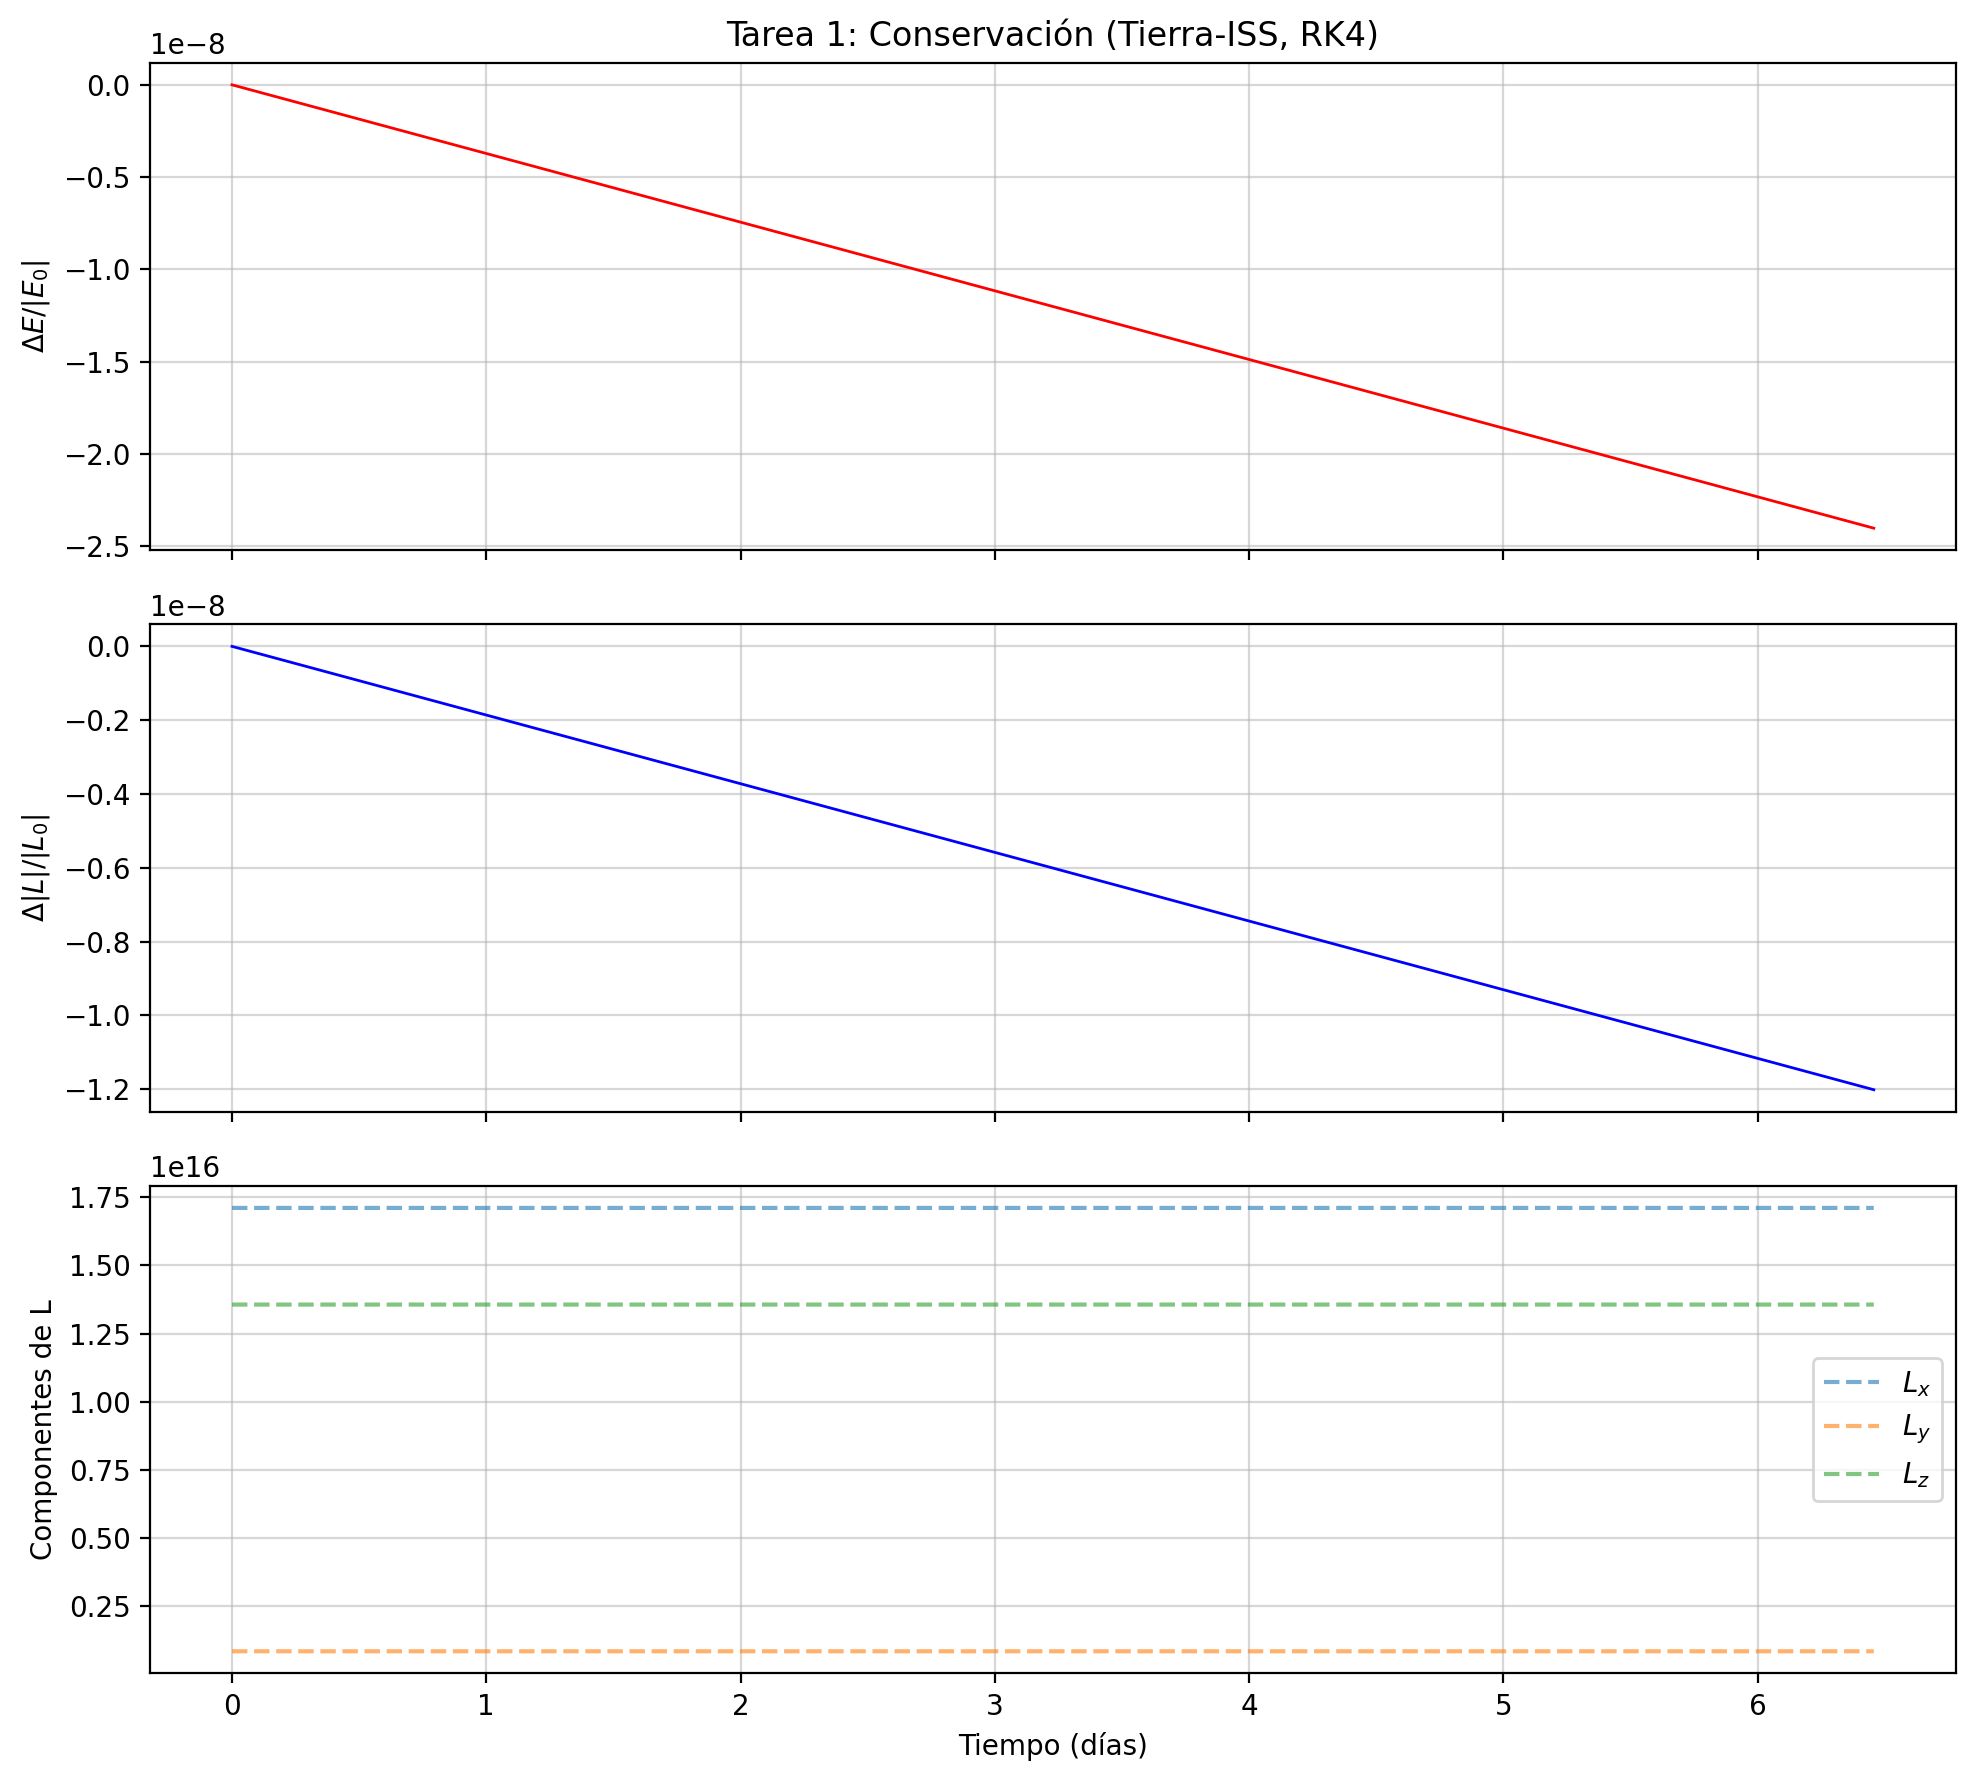
\includegraphics[width=0.75\textwidth]{T1v2_03_Conservacion.png}
	\caption{Validación Tarea 1 (RK4): deriva secular de energía $\Delta E/|E_0| = -2.4\times10^{-8}$ en 100 órbitas; $\Delta|L|/|L_0| = -1.2\times10^{-8}$.}
	\label{fig:t1_cons}
\end{figure}

\begin{figure}[H]
	\centering
	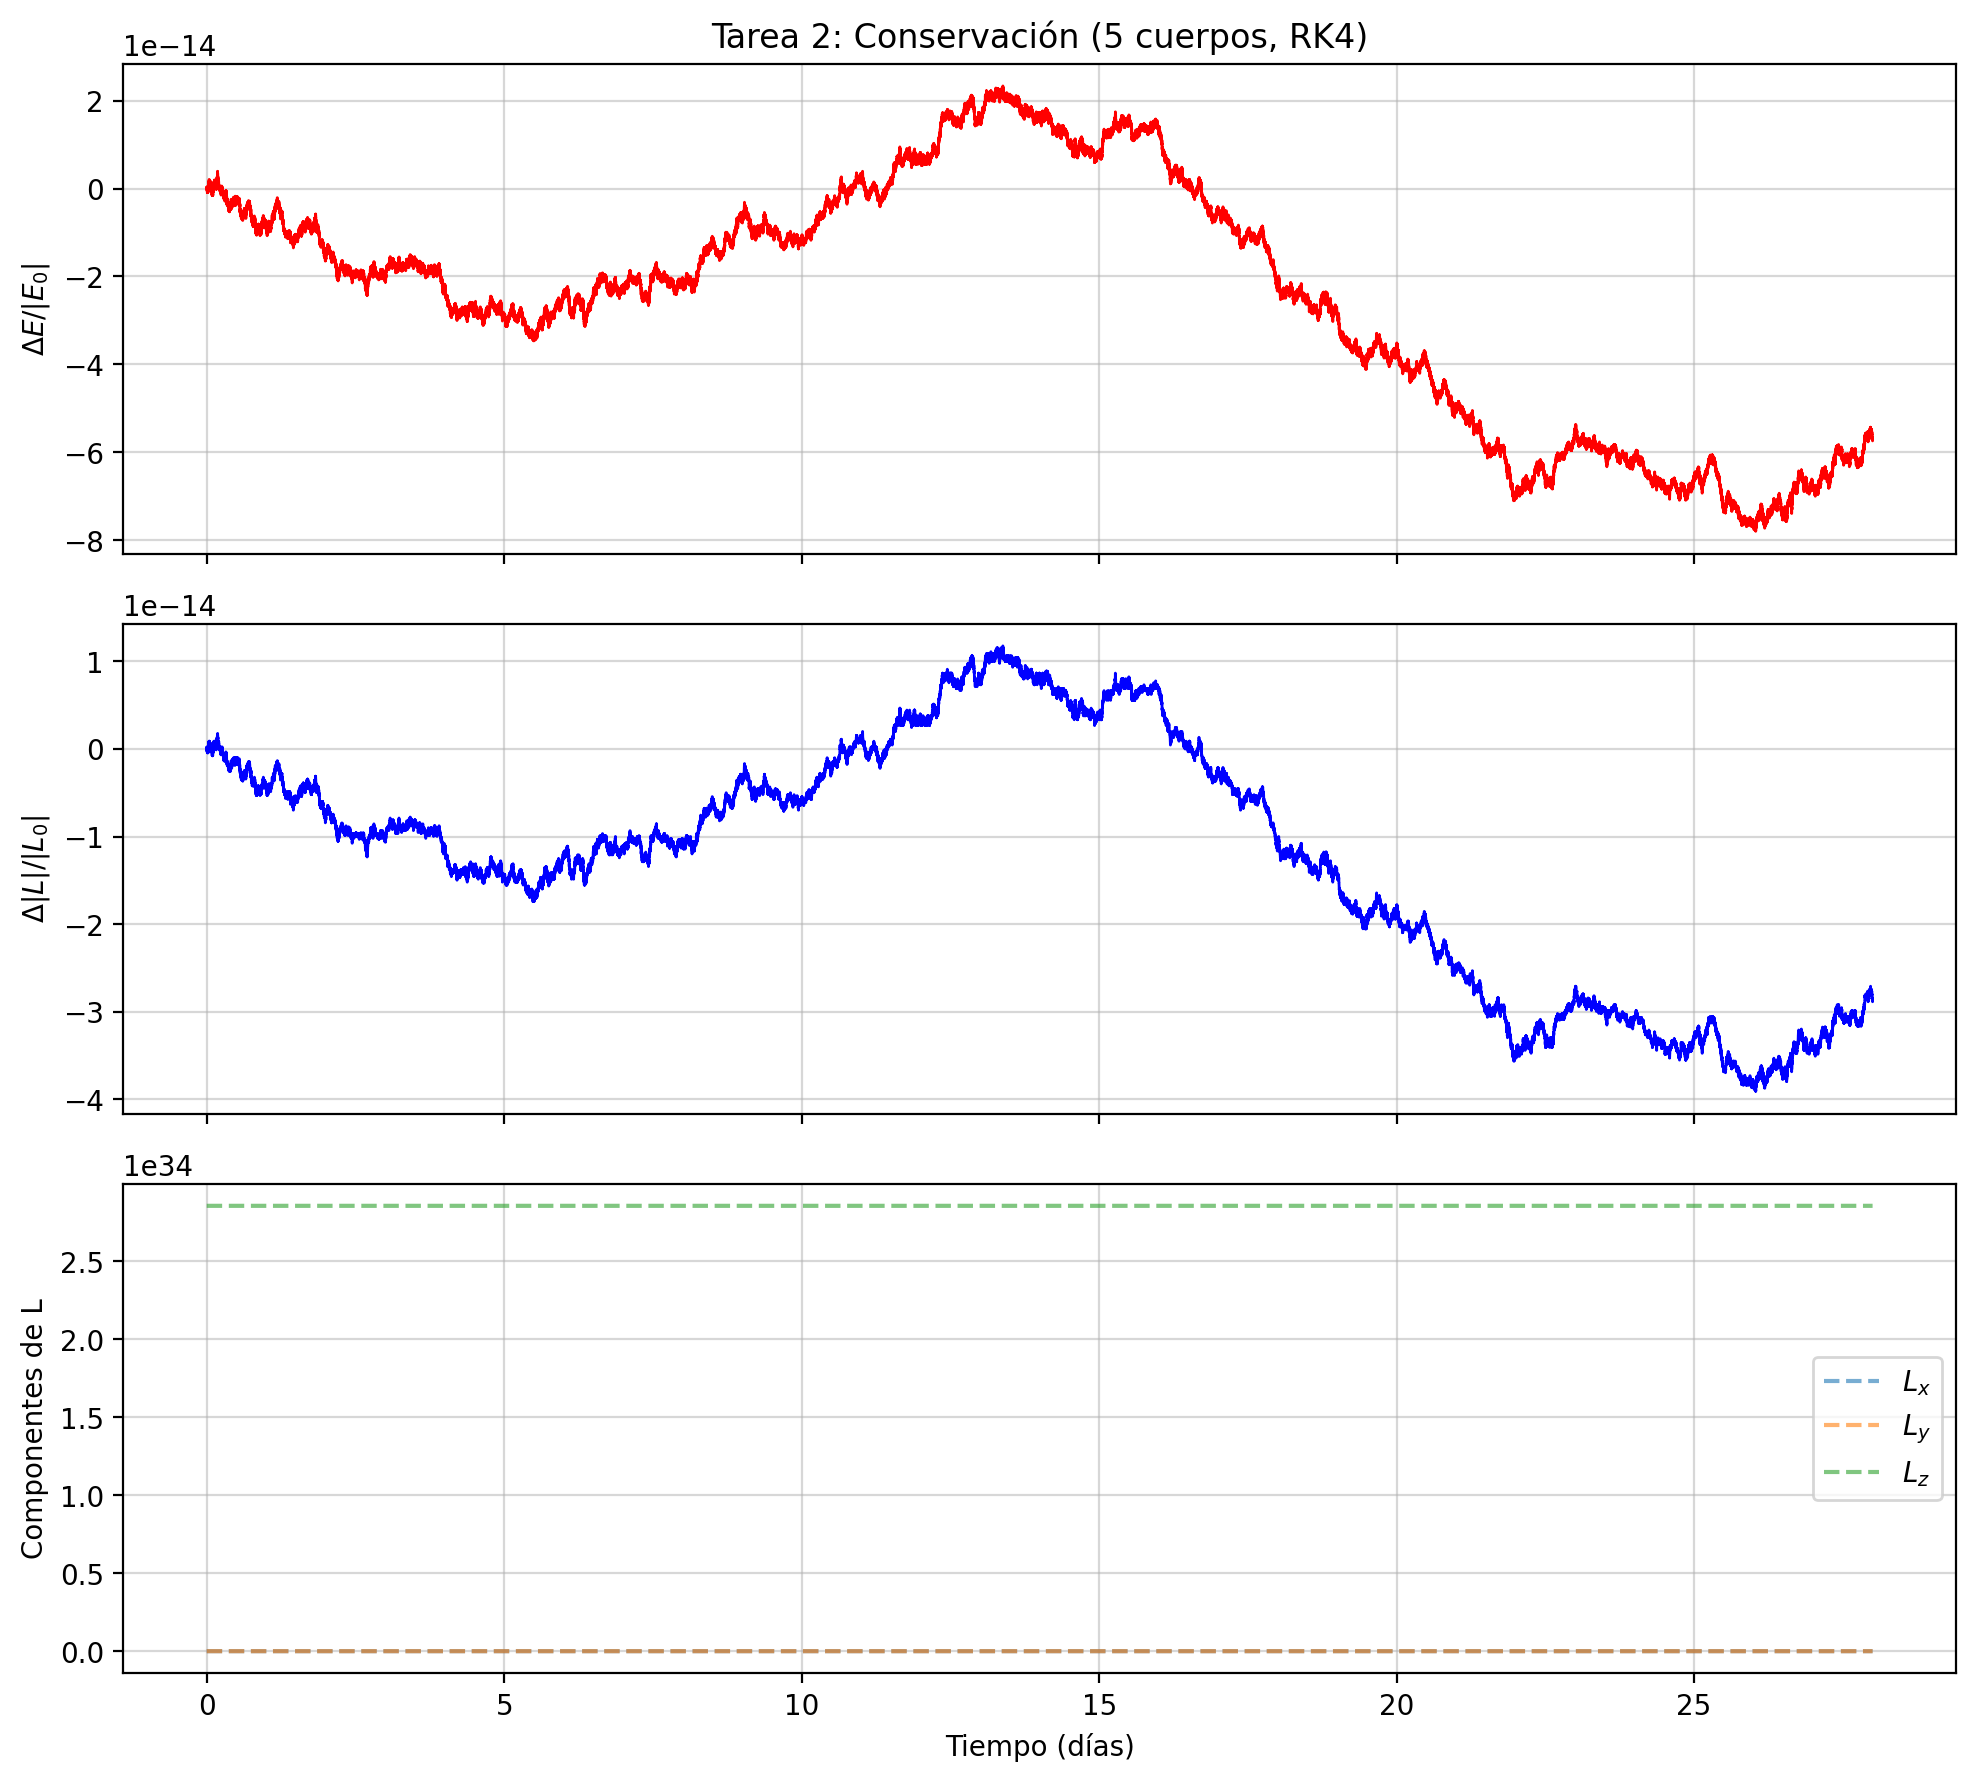
\includegraphics[width=0.75\textwidth]{T2v2_03_Conservacion.png}
	\caption{Validación Tarea 2 (RK4, 5 cuerpos): $\Delta E/|E_0| = -5.7\times10^{-14}$, $\Delta|L|/|L_0| = -2.9\times10^{-14}$ en 28 días.}
	\label{fig:t2_cons}
\end{figure}

\begin{figure}[H]
	\centering
	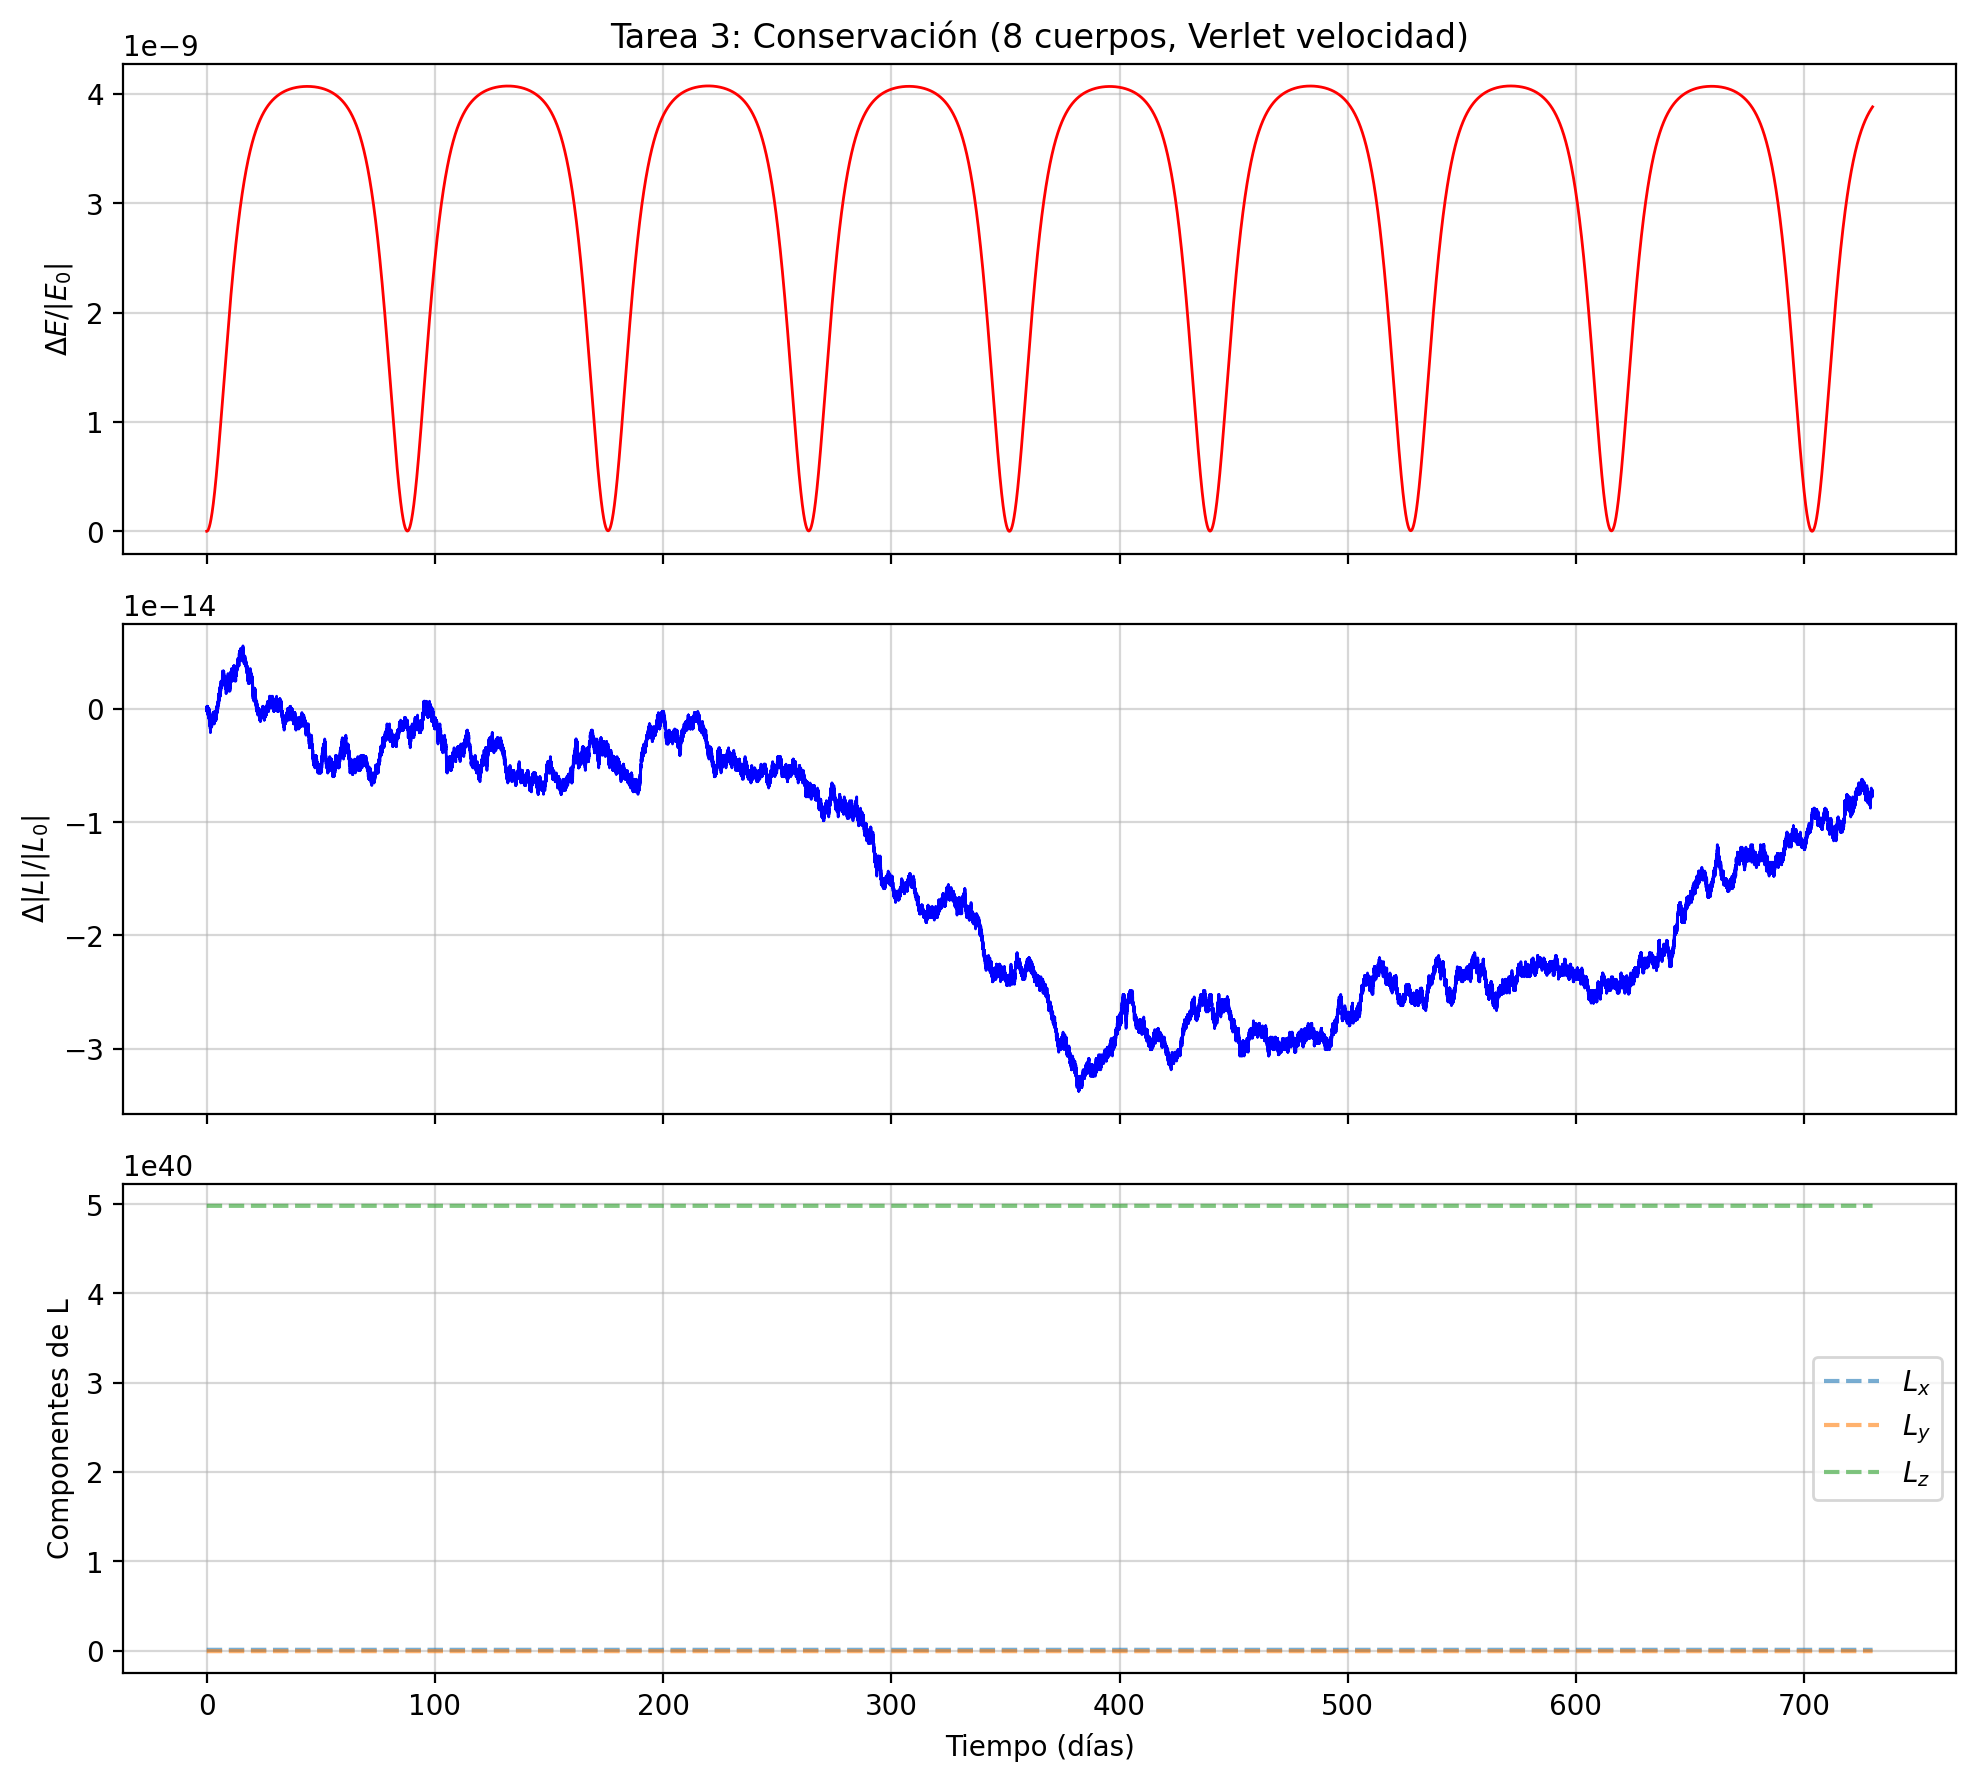
\includegraphics[width=0.75\textwidth]{T3v2_03_Conservacion.png}
	\caption{Validación Tarea 3 (Verlet velocidad, 8 cuerpos): la energía presenta \emph{oscilación acotada} $\max|\Delta E/E_0| = 4.1\times10^{-9}$ sin deriva secular (firma simpléctica), y $\Delta|L|/|L_0| < 3.4\times10^{-14}$.}
	\label{fig:t3_cons}
\end{figure}

El contraste entre integradores es el resultado central de la validación: RK4 disipa energía de forma secular (crecimiento lineal, Figs.~\ref{fig:t1_cons}--\ref{fig:t2_cons}), mientras que el esquema simpléctico la conserva en promedio con oscilación acotada (Fig.~\ref{fig:t3_cons}), sin deriva a pesar de integrar 105\,000 pasos. Esto justifica la elección de Verlet para la simulación de larga duración de la Tarea 3, tal como recomienda el enunciado. (Nótese que en sistemas multi-cuerpo el error relativo del sistema diluye el error del satélite de menor masa; por ello la métrica relativa de la Tarea 2 es más estricta de lo que aparenta.)

\subsection{Análisis Formal del Tamaño de Paso: Deriva Medida vs.\ Error Teórico}
\label{sec:analisis_h}

\subsubsection{Error teórico de truncamiento}
El error general de la primera derivada para un esquema de $n$ puntos, correspondiente a la Ec.~(0.6) del enunciado, es
\begin{equation}
	E'_n = \frac{h^n f^{(n+1)}(\xi)}{(n+1)!\, a_{0n}} \sum_{k=0}^n (k+1)\, a_{0k}\, s^k
	\label{eq:error_general}
\end{equation}
y para $n = 3$ (Ec.~(0.7) del enunciado):
\begin{equation}
	E'_3 = -\frac{h^3}{12} \left(3 - 11s + 9s^2 - 2s^3\right) f^{(iv)}(\xi)
	\label{eq:error_e3}
\end{equation}

\subsubsection{Cuarta derivada desde la ley de Newton}
Para una órbita cuasi-circular, $a = \ddot{r} = -\mu/r^2$; derivando dos veces respecto al tiempo y usando $v^2 \approx \mu/r$:
\begin{equation}
	f^{(iv)} = \frac{d^2a}{dt^2} = \frac{2\mu}{r^3}a - \frac{6\mu}{r^4}v^2 \approx -\frac{2\mu^2}{r^5} - \frac{6\mu^2}{r^5} = -\frac{8\,\mu^2}{r^5}
	\label{eq:f4}
\end{equation}
de modo que $|f^{(iv)}| \propto r^{-5}$: el cuerpo más interno domina el error.

\subsubsection{Deriva medida vs.\ cota teórica (Tarea 1)}
Se repitió el benchmark de 100 períodos con cuatro valores de $h$. La tabla compara la deriva final medida contra la cota teórica acumulada $N_{\text{pasos}} \times |E'_3|$ (con $s=1$ y $|f^{(iv)}|$ de la Ec.~(\ref{eq:f4}) para la ISS: $|f^{(iv)}| = 8.75\times10^{-5}\ \mathrm{m/s^4}$):

\begin{table}[H]
	\centering
	\begin{tabular}{rrrr}
		\toprule
		$h$ (s) & Deriva medida (m) & Cota $E'_3$ acumulada (m) & Razón medida/cota \\
		\midrule
		10  & $11.7$     & $406.9$    & $0.029$ \\
		15  & $84.9$     & $915.5$    & $0.093$ \\
		30  & $2\,590.1$ & $3\,662.0$ & $0.71$ \\
		60  & $80\,889.8$& $14\,647.9$& $5.52$ \\
		\bottomrule
	\end{tabular}
	\caption{Tarea 1: deriva del solver medida frente a la cota teórica de truncamiento (Ec.~\ref{eq:error_e3}) para distintos pasos.}
	\label{tab:drift}
\end{table}

\begin{figure}[H]
	\centering
	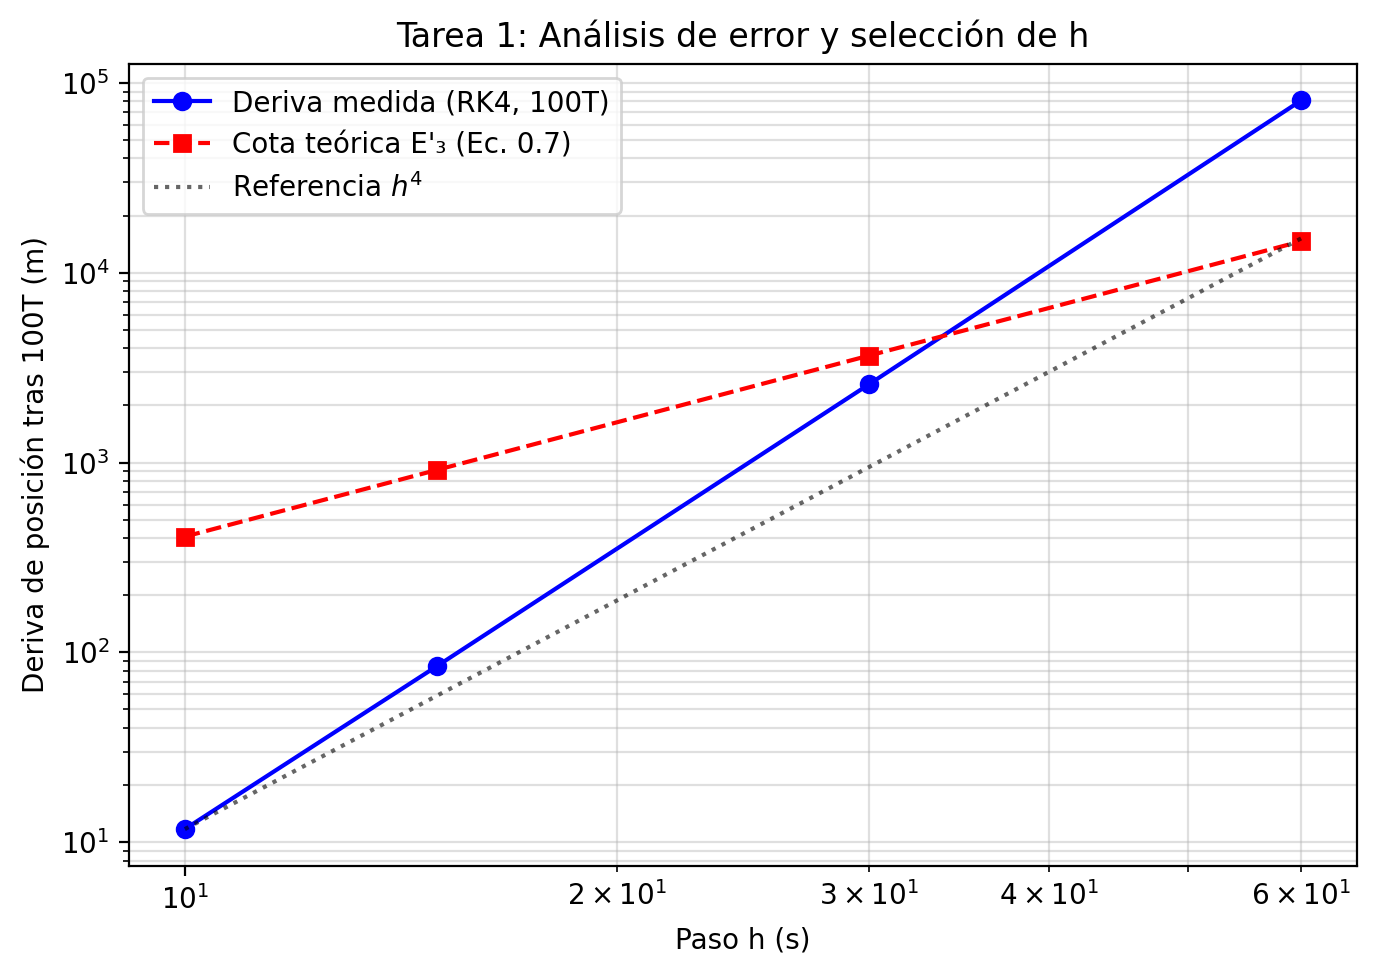
\includegraphics[width=0.62\textwidth]{T1v2_04_Barrido_h.png}
	\caption{Tarea 1: escalado de la deriva medida con $h$ (pendiente log-log $p = 4.94$), la cota $E'_3 \propto h^3$ (acumulada $\propto h^2$) y la referencia $h^4$ (orden global de RK4).}
	\label{fig:t1_barrido}
\end{figure}

\textbf{Lectura de resultados}: la deriva medida escala con pendiente log-log $p = 4.94$, consistente con el orden global $h^4$ de RK4 (la componente secular along-track puede elevar ligeramente el exponente efectivo). Para $h \le 30$ s la deriva medida permanece \emph{por debajo} de la cota $E'_3$, que actúa como cota conservadora del régimen lineal; para $h = 60$ s el crecimiento $h^{4.94}$ del error real de RK4 supera la cota (que acumulada crece solo $\propto h^2$). La elección $h = 15$ s queda así justificada con doble margen: deriva medida de 84.9 m ($< 0.001$ del radio orbital) en 100 órbitas y cota teórica de $0.92$ km.

\subsubsection{Justificación de $h$ por tarea}
Aplicando el criterio ``el cuerpo con mayor $|f^{(iv)}|$ define el $h$ de todo el sistema'':

\begin{table}[H]
	\centering
	\begin{tabular}{llrrl}
		\toprule
		Tarea & Cuerpo crítico & $|f^{(iv)}|$ (m/s$^4$) & $h$ elegido (s) & $E'_3$ por paso \\
		\midrule
		1--2 & ISS ($a = 6.798\times10^6$ m)   & $8.75\times10^{-5}$ & 15  & $2.5\times10^{-2}$ m \\
		3    & Fobos ($r = 9.38\times10^6$ m)  & $2.02\times10^{-7}$ & 600 & $3.6$ m \\
		3    & Mercurio ($r = 5.79\times10^{10}$ m) & $2.2\times10^{-13}$ & --- & despreciable \\
		\bottomrule
	\end{tabular}
	\caption{Cuerpo crítico por tarea según la Ec.~(\ref{eq:f4}) y error de truncamiento asociado al paso elegido.}
	\label{tab:h_por_tarea}
\end{table}

\textbf{El cuerpo crítico de la Tarea 3}: \emph{no es Mercurio sino Fobos}, cuya órbita de período $7.65$ h alrededor de Marte es la de mayor frecuencia del sistema. Con un paso grueso de $h = 3600$ s, Fobos se muestrearía con solo $\approx 7.6$ puntos por órbita y el error de truncamiento acumulado sería
\begin{equation}
	h = 3600\ \mathrm{s}: \quad E'_3 = 787\ \mathrm{m/paso} \times 17\,520\ \mathrm{pasos} \approx 13\,800\ \mathrm{km} \; > \; r_{\text{orbital}} = 9\,377\ \mathrm{km},
\end{equation}
es decir, la órbita quedaría numéricamente corrupta. Con $h = 600$ s ($\approx 46$ muestras por órbita de Fobos) la cota acumulada cae a $\approx 383$ km ($\sim 4\%$ del radio orbital), aceptable para un análisis del sistema planetario; esta es la elección adoptada. Análogamente, en las Tareas 1--2 la presencia de la ISS en LEO obliga a mantener $h = 15$ s aunque la Luna y el punto $L_2$ tolerarían pasos mucho mayores.

\subsection{Resumen numérico de validación}

\begin{table}[H]
	\centering
	\begin{tabular}{llll}
		\toprule
		Tarea & Integrador & $\max|\Delta E/E_0|$ & $\max \Delta|L|/|L_0|$ \\
		\midrule
		T1: Tierra-ISS (100 órbitas)   & RK4            & $2.4\times10^{-8}$ (secular) & $1.2\times10^{-8}$ \\
		T2: 5 cuerpos (28 días)        & RK4            & $5.7\times10^{-14}$          & $2.9\times10^{-14}$ \\
		T3: 8 cuerpos (730 días)       & Verlet vel.    & $4.1\times10^{-9}$ (acotada) & $3.4\times10^{-14}$ \\
		\bottomrule
	\end{tabular}
	\caption{Conservación de energía y momento angular por tarea. La distinción ``secular'' vs.\ ``acotada'' distingue el comportamiento disipativo de RK4 del comportamiento simpléctico.}
	\label{tab:conservacion}
\end{table}

% ==============================================================================
\section{Conclusiones}
% ==============================================================================

\begin{enumerate}
	\item Se construyó un motor de simulación $N$-cuerpos modular y vectorizado, con dos integradores propios (RK4 y Verlet velocidad), interpolación de Lagrange, detección de eventos por bisección (verificada con la constante 2.667) y registro completo de estados y magnitudes conservadas.
	\item El benchmark analítico de 2 cuerpos con TLE real de la ISS midió una deriva de 84.9 m en 100 órbitas con $h = 15$ s, con escalado $h^{4.94}$ consistente con el orden global de RK4, y por debajo de la cota de truncamiento $E'_3$ en todo el régimen útil.
	\item El sistema restringido Tierra-Luna mostró numéricamente la estabilidad de $L_4$ (libación acotada) frente a la inestabilidad exponencial de $L_2$, en acuerdo con la teoría del potencial efectivo co-rotante.
	\item La expansión a 8 cuerpos reprodujo la inclinación de $7^\circ$ de Mercurio y permitió medir su precesión secular newtoniana ($148.7''$/siglo con los planetas interiores, orden de magnitud consistente con la teoría secular) y su regresión nodal ($-471''$/siglo). La comparación 2D vs.\ 3D demostró que el modelo planar sobreestima la precesión por un factor $\sim 6.6$ al suprimir los grados de libertad fuera del plano.
	\item La validación física distinguió claramente la deriva secular de energía de RK4 de la oscilación acotada del integrador simpléctico ($4\times10^{-9}$ en 105\,000 pasos), confirmando la preferencia del enunciado por esquemas simplécticos en simulaciones de larga duración.
	\item El análisis de truncamiento identificó a Fobos ---no a Mercurio--- como el cuerpo crítico de la Tarea 3, justificando cuantitativamente la elección del paso $h = 600$ s frente a valores más gruesos que corromperían numéricamente su órbita.
\end{enumerate}

% ==============================================================================
\begin{thebibliography}{9}

\bibitem{kopeikin2011}
Kopeikin, S., Efroimsky, M. y Kaplan, G. (2011). \textit{Relativistic Celestial Mechanics of the Solar System}. Wiley-VCH.

\bibitem{binney2008}
Binney, J. y Tremaine, S. (2008). \textit{Galactic Dynamics} (2.ª ed.). Princeton University Press.

\bibitem{murray1999}
Murray, C. D. y Dermott, S. F. (1999). \textit{Solar System Dynamics}. Cambridge University Press.

\bibitem{celestrak}
Celestrak (2026). \textit{GP Data / TLE, ISS (ZARYA), NORAD 25544}. Época 26282.82140207 (9 de octubre de 2026, 19:42 UTC). \url{https://celestrak.org/NORAD/elements/gp.php?CATNR=25544}

\bibitem{vallado2013}
Vallado, D. A. (2013). \textit{Fundamentals of Astrodynamics and Applications} (4.ª ed.). Microcosm Press. (Formato y reducción de TLE.)

\bibitem{newton1687}
Newton, I. (1687). \textit{Philosophiae Naturalis Principia Mathematica}.

\end{thebibliography}

\end{document}
